\chapter{Multi-Modal Simulation}
\label{ch:multimodalsim}
% ##################################################################################################################

\hfill \textbf{Authors:} Christoph Dobler, Gregor L�mmel

\begin{center} 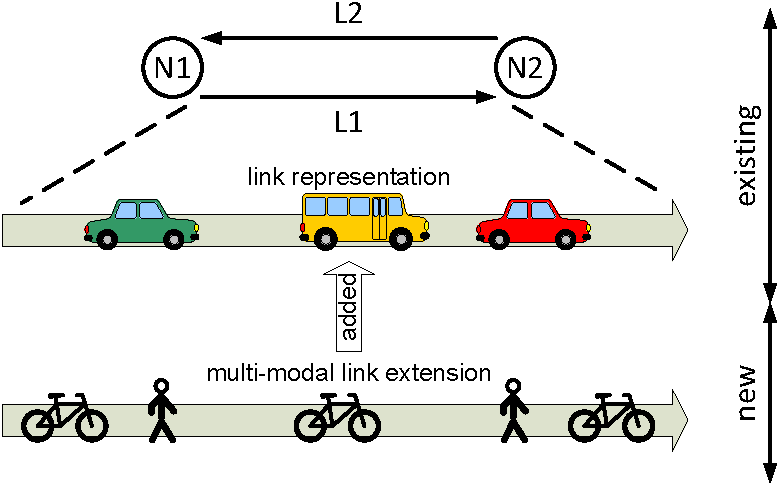
\includegraphics[width=0.5\textwidth, angle=0]{extending/figures/MultiModalSimulation/multi-modal-link-extension} \end{center}

% ##################################################################################################################

\textit{Parts of this chapter are based on work published at the 6th International Conference on Pedestrian and Evacuation Dynamics in Zurich  \citep{DoblerLaemmel_PED_2012}}.


% ##################################################################################################################
\section{Introduction}
Today, the field of application for agent-based traffic flow micro-simulations is widespread. Traditionally, those simulations were focused on large-scale vehicular traffic and produced information like average traffic flows and travel times. A subset of those applications, which has gained importance over the past years, are agent-based multi-modal simulations. In such models, various transport modes are simulated simultaneously, including the interactions between agents using different modes. Due to the agent-based simulation approach, each person in a scenario is represented as a single entity. Therefore, the movement of each single person can be tracked in detail, which is one essential requirement for studies related to topics like evacuations, e-bikes, car sharing or public transport.

Another even more important requirement for such studies is a simulation model's ability to also simulate non-vehicular traffic. Having a look at today's agent-based transport simulations shows that there are two basic types of simulation models available. The first type has been developed for large-scale scenarios with hundreds of thousands or even several million entities. To keep their computational effort acceptable, they are based on simplified physical representations of traffic flows as they are known from the field of dynamic traffic assignment. In contrast, the second type of model offers a high level of detail and a microscopic modelling of the underlying physics for small scenarios with some hundred or a few thousand agents. While the first class only deals with vehicular traffic, the second one usually also deals with pedestrians and cyclists.

An approach to reduce the gap between these two simulation types is presented in the following. To do so, the proposed multi-modal simulation model adds support for ride trips and non-motorized (i.e.~walk and bike) traffic to a framework for large-scale simulations. The next section discusses the requirements that those multi-modal extension has to fulfil. Afterwards, the modelling approaches for non-motorized and ride trips as well as their implementation in MATSim are described. Finally, the implementations are tested by conducting experiments with a sample scenario.

% ##################################################################################################################
\section{Requirements}
To be able to perform studies as mentioned above (evacuations, e-bikes, etc.), a multi-modal traffic flow simulation has to provide additional information compared to a simulation which only simulates vehicular traffic. As most important requirement, an agent's position has to be known during the entire simulated period. Common micro-simulations which only focus on vehicular traffic cannot provide this information. They either totally ignore non-motorized trips or teleport agents from origins to destinations of their trips. When using the latter approach, as MATSim does so far, travel times are often determined using simple estimation rules, e.g.~using an average travel speed and an estimated travelled distance based on the trip's crow-fly distance.

An application's required level of detail highly influences the selection of a modelling approach. A simple model which respects agents' age and gender but does not incorporate agent-agent interactions might be detailed enough for some studies (e.g.~e-bikes or public transport). However, for some other studies a more detailed model which also simulates agent interactions might be necessary (e.g.~evacuation of crowded pedestrian areas).

A model's computational effort increases with its level of detail. Therefore, to keep computation times short, a model should only be as detailed as necessary. On one hand, this can be realized by providing several models with various levels of detail and selecting an appropriate one. On the other hand, a flexible model with an adaptive level of detail can be used. While the latter ones are more complex, they can in turn  be more detailed where needed and more aggregated where possible.

One of very few implementations of a model with different levels of detail is presented by \citet{SewallJEtAl_ACMTG_2011}. They use a hybrid model of both continuum and agent-based methods for vehicular traffic simulations. In regions of interest, the simulation uses an agent-based approach, in the remaining parts a faster continuum model.

For some applications it is necessary that agents using different transport modes can interact. When modelling such interactions it is in general meaningful that infrastructure which would be shared in the real world is also shared in the simulation. Doing so simplifies keeping the simulation's behaviour consistent. An example is the simulation of shared trips. When sharing infrastructure, an agent which performs a ride trip physically enters a vehicle and reduces its free capacity. Therefore, the agent has to wait until the vehicle has arrived and then check whether it has free capacity left. Moreover, the vehicle can wait at the meeting point if the agent to be picked up has not yet arrived.

When not sharing infrastructure, the simulation module for ride trips has to observe all vehicles and track their passengers and capacities. However, a vehicle will not recognize when a passenger has not yet arrived because it does not communicate with the ride simulation module. As a result, the vehicle will depart and the passenger will not be able to perform its scheduled ride trip. An advantage of this approach is that a ride simulation module could be developed without changing code in the vehicular simulation module.

Compared to vehicular traffic flow simulations, non-vehicular simulations require different input data. An agent's age and gender, for example, highly influences its walk speed, but is not taken into account by models for vehicular traffic flows. Models which include agent-agent or agent-environment interactions additionally need detailed information related to the road network's geometry (e.g.~shape, width and height profile of links) as well as buildings and other obstacles in the simulated area.

% ##################################################################################################################
\section{Modelling Approach and Implementation}
\subsection{Multi-modal Link Extension} \label{sec:Multi-modalSimulation}
For the simulation of non-motorized trips a new simulation module has been developed for MATSim's \emph{QSim}. Figure \ref{fig:multi-modal-link-extension} shows the implementation's basic concept---a multi-modal extension is added to each link object in the mobility simulation. By doing so, the existing network infrastructure is re-used, which---as discussed before---simplifies the realization of interactions between agents using different transport modes.

%---------------------------------------------------------------------
\createfigure%
{Multi-modal link extension}%
{Multi-modal link extension}%
{\label{fig:multi-modal-link-extension}}%
{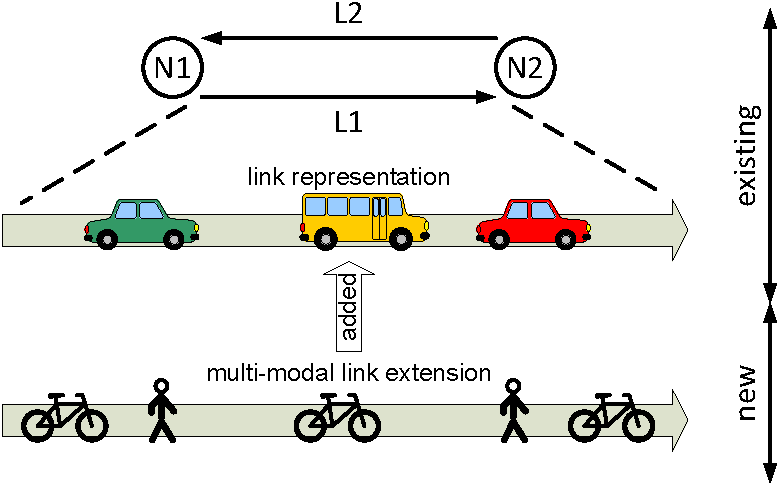
\includegraphics[width=0.75\textwidth, angle=0]{extending/figures/MultiModalSimulation/multi-modal-link-extension}}%
{}
%---------------------------------------------------------------------

While traffic flow dynamics are simulated by MATSim's mobility simulation using a queue model, they are not taken into account in the multi-modal extension. Having a look at typical pedestrian and cyclist traffic flows shows that congestion is very rare compared to vehicular traffic and therefore justifies the application of this simplistic approach in large parts of a scenario. For regions with higher traffic flows, this simple model looses accuracy but still outperforms the teleportation approach which MATSim uses by default.

Each multi-modal link extension uses a priority queue to manage all agents travelling on that link using a non-motorized mode. The queue orders the agents based on their scheduled link leave time (see Figure \ref{fig:linkRepresentationSimpleModel}). This time is calculated when an agent enters a link based on parameters like the agent's age and gender as well as the links steepness. In each time step it is checked, whether the queue contains agents who have reached their link leave time and therefore have to be moved to their route's next link. An agent's position on a link is not determined by the model. However, under the assumption that agents move with constant speed, their position can be interpolated. This approach is computationally very efficient because computation effort is only created when an agent enters or leaves a link but not when the agent is travelling along a link. Additionally, agents can travel with different speeds and therefore overtake each other.

%---------------------------------------------------------------------
\createfigure%
{Link representation in the simple model}%
{Link representation in the simple model. \\At time~12084, agent~512 enters the link and is---based on its calculated link leave time 14618---inserted into the queue. At time~12312, agent~780 has reached its leave time and therefore is removed from the queue.}%
{\label{fig:linkRepresentationSimpleModel}}%
{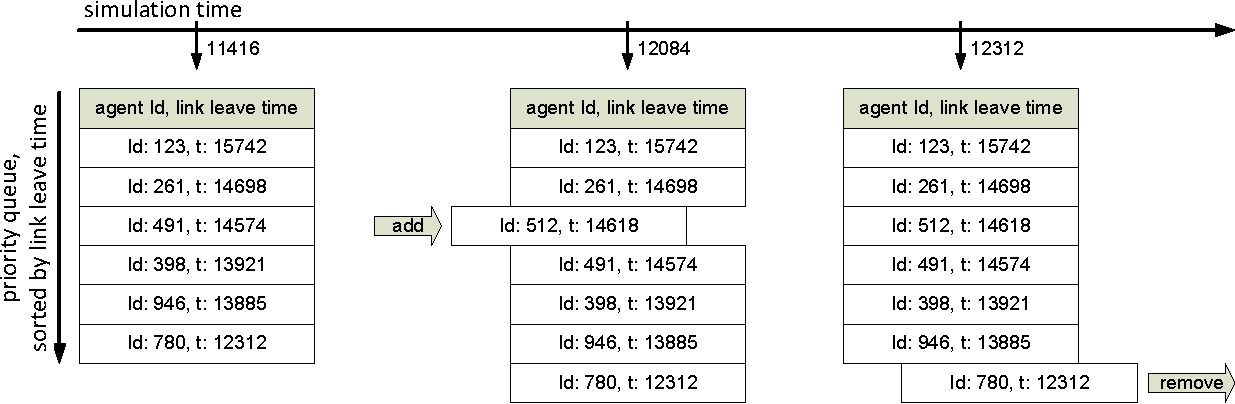
\includegraphics[width=1.0\textwidth, angle=0]{extending/figures/MultiModalSimulation/linkRepresentation}}%
{}
%---------------------------------------------------------------------

To increase the simulation's accuracy in crowded regions, models which are able to simulate interactions between agents and their environment (other agents but also other obstacles like buildings or parked vehicles) can be applied. A large group of models doing so are based on a force-based approach. There, agents' movement is based on additive attracting and repelling forces, which are ``pushing'' the agents through the environment.

In recent years, many different force-based models have been introduced and discussed. An overview is e.g.~given by \citet{OlesonEtAl_BazzanKluegl_2009}. Most of those models are build on the so-called social force model introduced by \citet{HelbingMolnar_PhysRevE_1995}. Collision avoiding behaviour---as it can be observed in real-world situations---is implicitly reproduced by the basic social force model. It has been shown that the model works particularly well in high density conditions, such as one can observe in evacuation situations \citep{HelbingEtAl_Nature_2000}.

\citet{LaemmelPlaue_PED_2012} present an experimental implementation of a pedestrian simulation module for MATSim based on a force-base model. The agents' high-level planning (i.e.\ route and destination choice) is performed on a graph representing the transport system (e.g.~a MATSim network) while the low level behaviour (i.e. physical interaction between the participants) is simulated with a force-based model. Besides agent-agent interactions, also interactions between agents and other obstacles are simulated. To do so, additional input data like the road network's geometry and building limits is required. Unfortunately, the scenario size is limited to a few thousand agents due to the model's high computational effort. An attempt to bypass this limitation is presented by \citet{DoblerLaemmel_PED_2012}. They combine the force-based pedestrian simulation module with the multi-modal link extension. Doing so gives the opportunity to simulate large-scale scenarios, while staying highly resolved where needed and being more aggregated where possible.

%---------------------------------------------------------------------
\subsection{Travel Times} \label{sec:TravelTimes}
Walk travel time calculation is based on results of a comprehensive literature review presented by \citet{Weidmann_TechRep_IVT_1992}. Starting point is a normally distributed reference speed of 1.34~m/s with a standard deviation of 0.26~m/s, which leads to an individual reference speed for each person. \citet{HBS_2009} and \citet{HCM_2010} report comparable but not as detailed data. If a trip's purpose is known, a person's reference value can be adjusted \citep[commuting 1.49~m/s, shopping 1.16~m/s, leisure 1.10~m/s; see][]{HBS_2009}. Using the reference speed and respecting a person's age, gender and statistical spreading, a personalized speed is calculated (see Figure \ref{fig:labelPedestriansAge}). Finally, to calculate the person's travel time on a specific link, the influence of the link's steepness on the person's speed is taken into account (see Figure \ref{fig:labelPedestriansSteepness}). The combination of person specific attributes and link steepness is shown in Figure \ref{fig:labelPedestriansAgeSteepness3d}.

As a result, a person's speed on plain terrain is calculated as:\begin{align}
	f\textsubscript{person} = f\textsubscript{statistical~spreading} \cdot f\textsubscript{gender} \cdot f\textsubscript{age}\\
	v\textsubscript{person, walk} = v\textsubscript{reference, walk} \cdot f\textsubscript{person}
\end{align}
A link's steepness is incorporated as:
\begin{align}
    v\textsubscript{person~walks~on~link} &= v\textsubscript{person, walk} \cdot f\textsubscript{steepness}
\end{align}

%---------------------------------------------------------------------
\createfigure%
{Age and steepness dependent speed of pedestrians}%
{Age and steepness dependent speed of pedestrians}%
{\label{fig:labelWalkTravelTimes}}%
{%
  \createsubfigure%
  {Age dependent speed}%
  {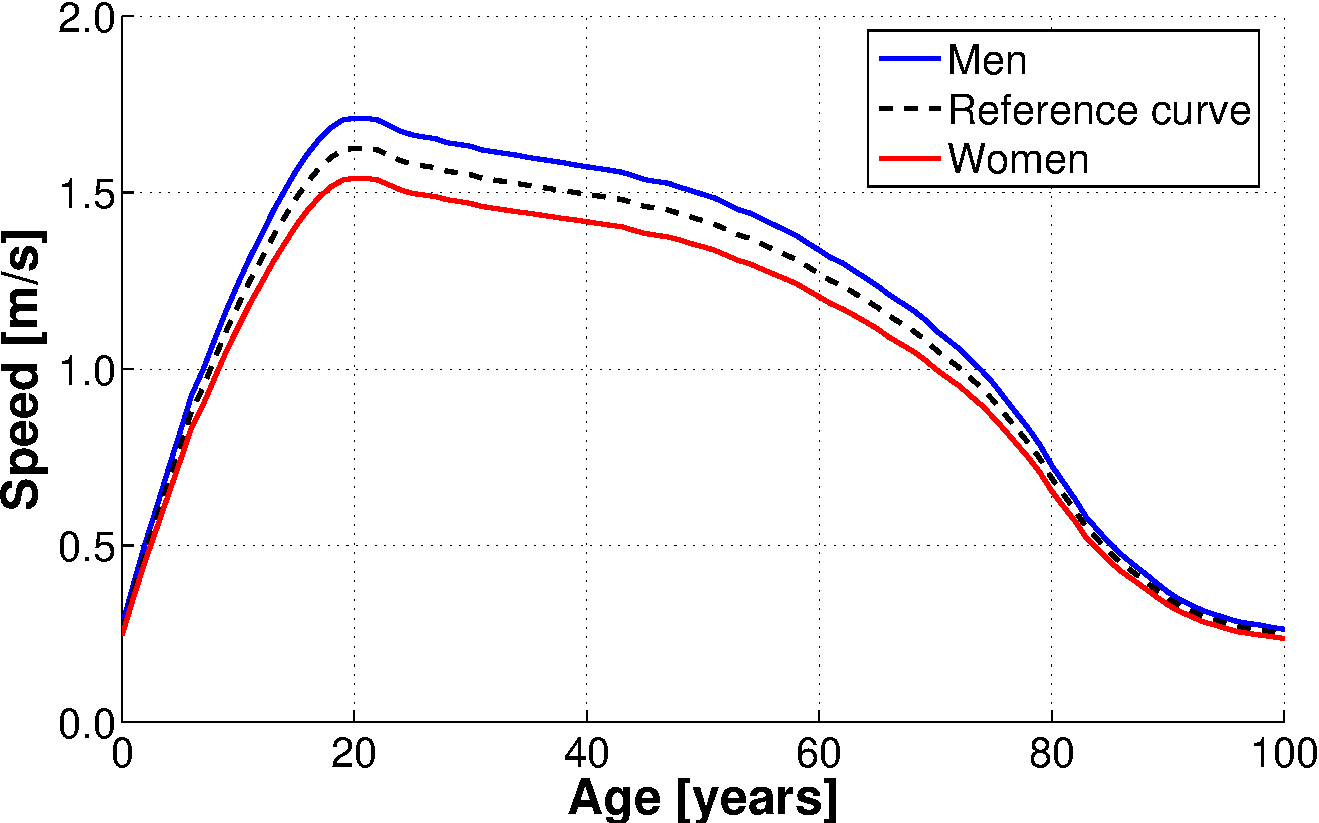
\includegraphics[width=0.70\textwidth, angle=0]{extending/figures/MultiModalSimulation/pedestriansAge}}%
  {\label{fig:labelPedestriansAge}}%
  {\vspace{3mm}}%

  \createsubfigure%
  {Steepness dependent speed}%
  {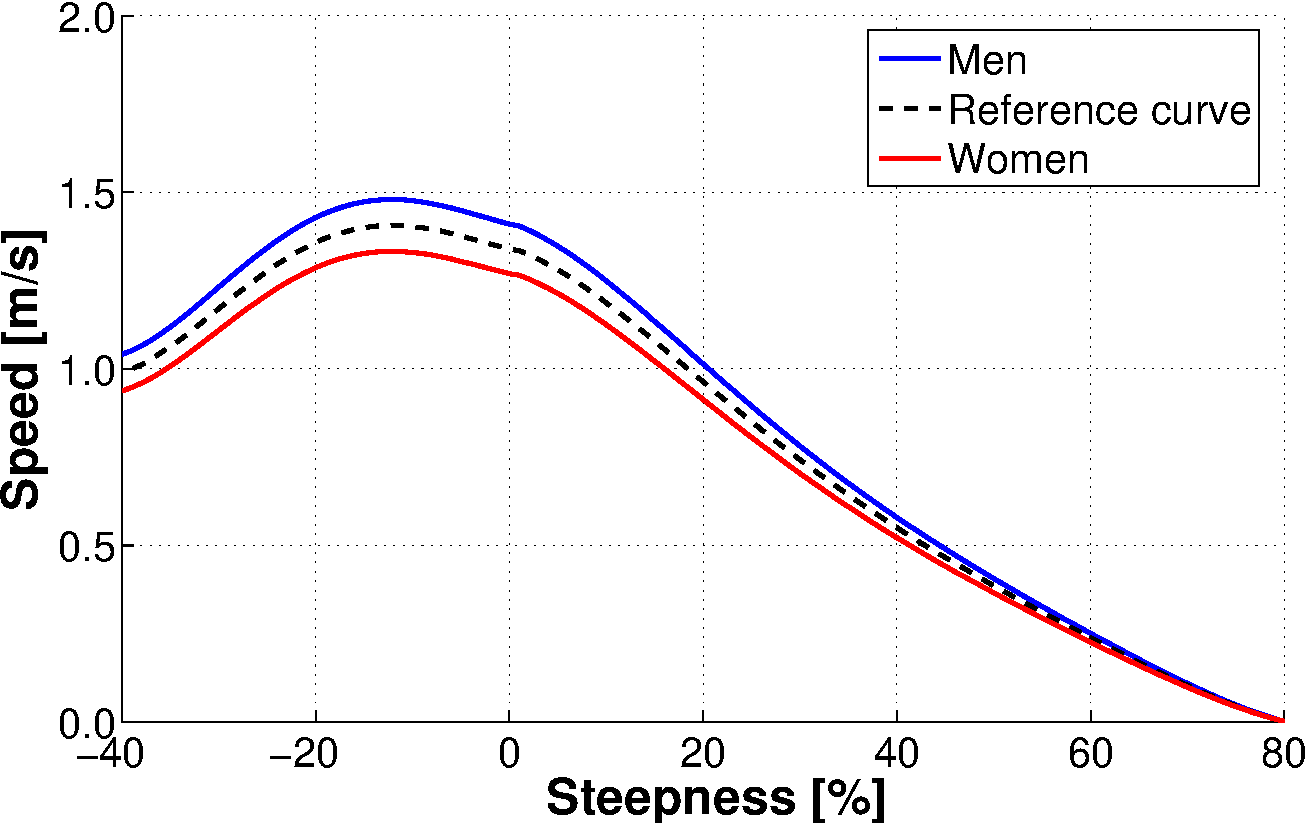
\includegraphics[width=0.70\textwidth, angle=0]{extending/figures/MultiModalSimulation/pedestriansSteepness}}%
  {\label{fig:labelPedestriansSteepness}}%
  {\vspace{3mm}}%

  \createsubfigure%
  {Age and steepness dependent speed}%
  {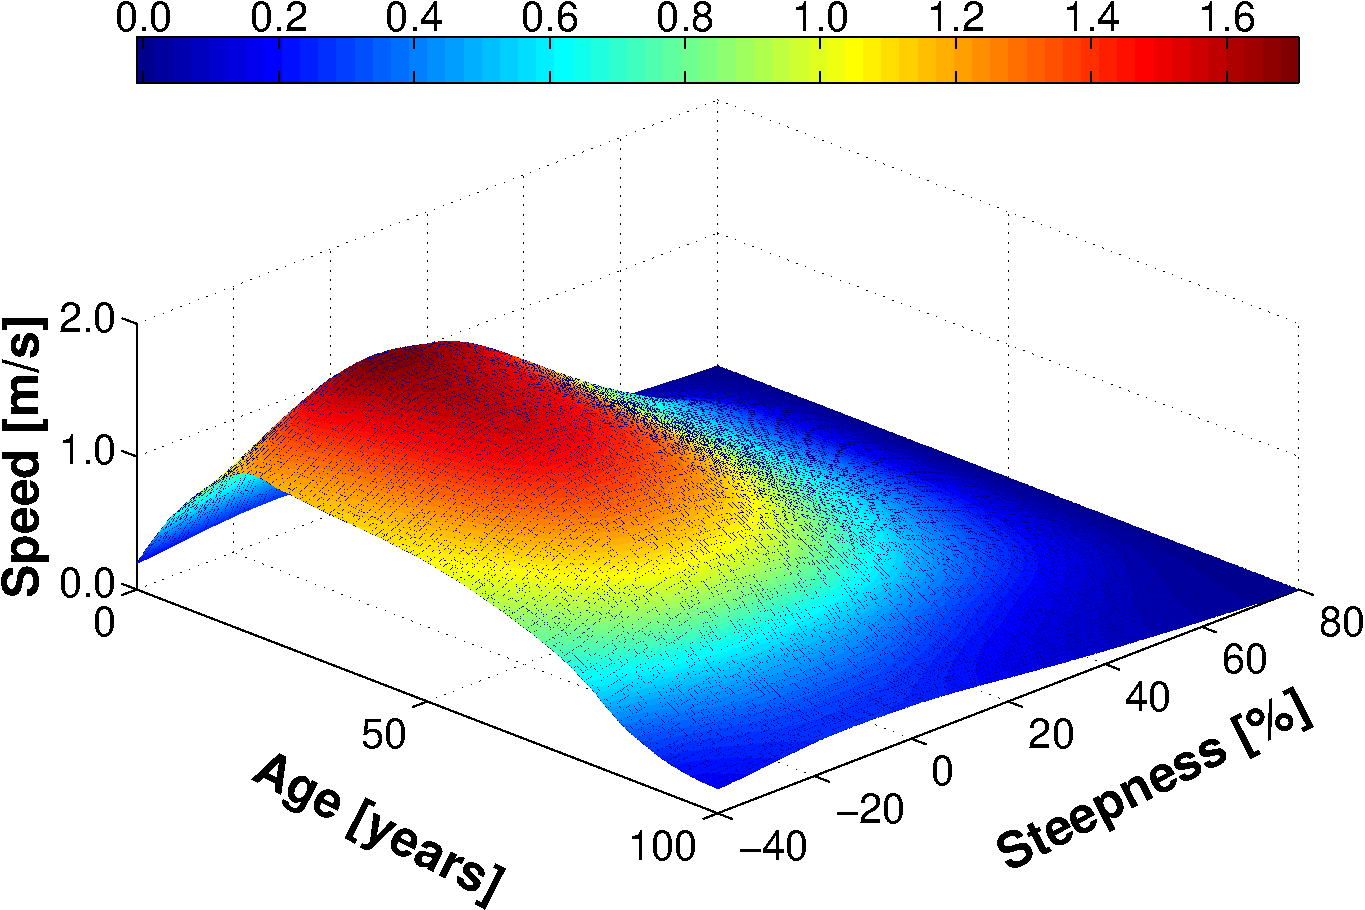
\includegraphics[width=0.70\textwidth, angle=0]{extending/figures/MultiModalSimulation/pedestrians3d}}%
  {\label{fig:labelPedestriansAgeSteepness3d}}%
  {}%
}%
{}
%---------------------------------------------------------------------

The speed of cyclists is determined using results from \cite{ParkinRotheram_TPol_2010}. Starting point is again an individual's speed based on a normal distributed ($\mathcal{N}(6.01,1.17)$) reference speed. Again, a person's speed is calculated by accounting for age and gender (see Figure \ref{fig:labelCyclistsAge}).

%---------------------------------------------------------------------
\createfigure%
{Age and steepness dependent speed of cyclists}%
{Age and steepness dependent speed of cyclists}%
{\label{fig:labelBikeTravelTimes}}%
{%
  \createsubfigure%
  {Age dependent speed}%
  {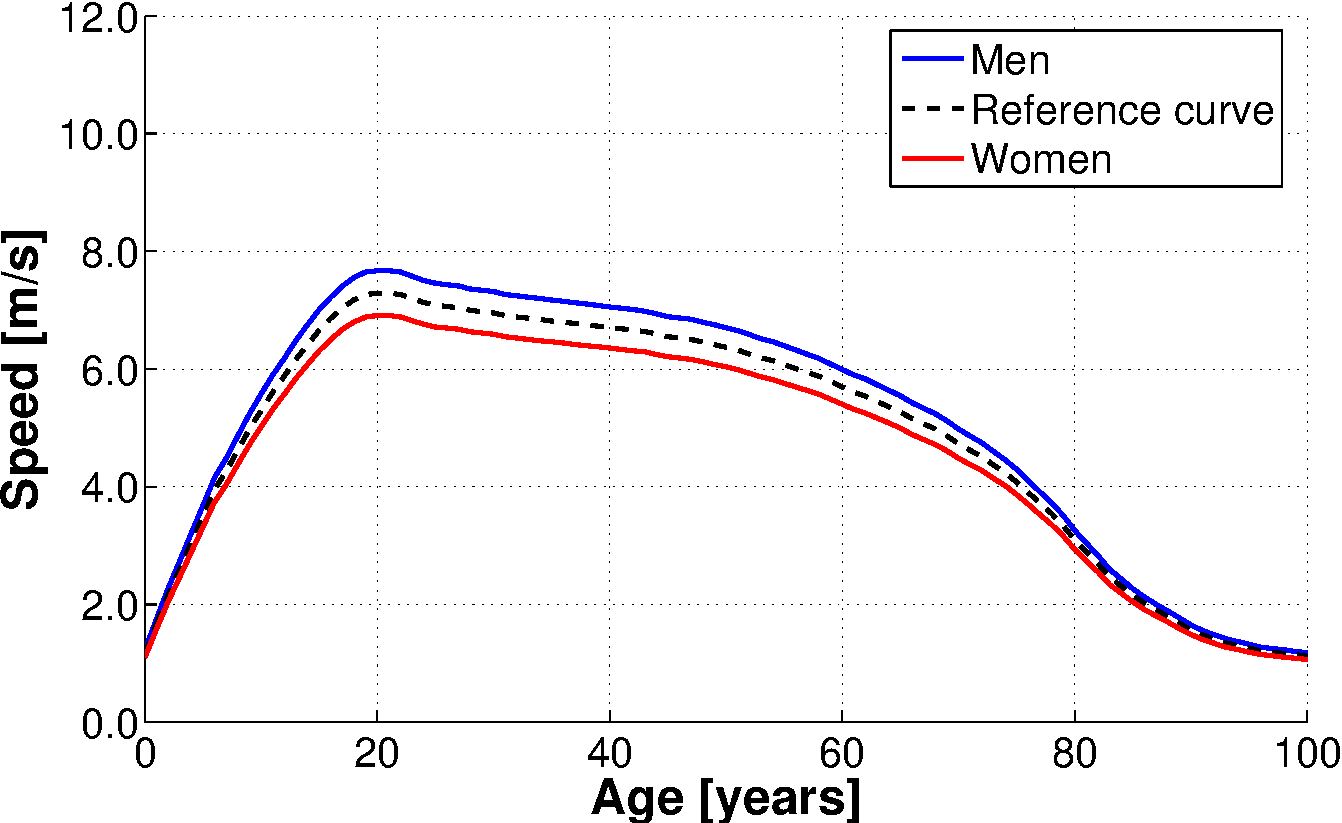
\includegraphics[width=0.70\textwidth, angle=0]{extending/figures/MultiModalSimulation/cyclistsAge}}%
  {\label{fig:labelCyclistsAge}}%
  {\vspace{5mm}}%

  \createsubfigure%
  {Steepness dependent speed}%
  {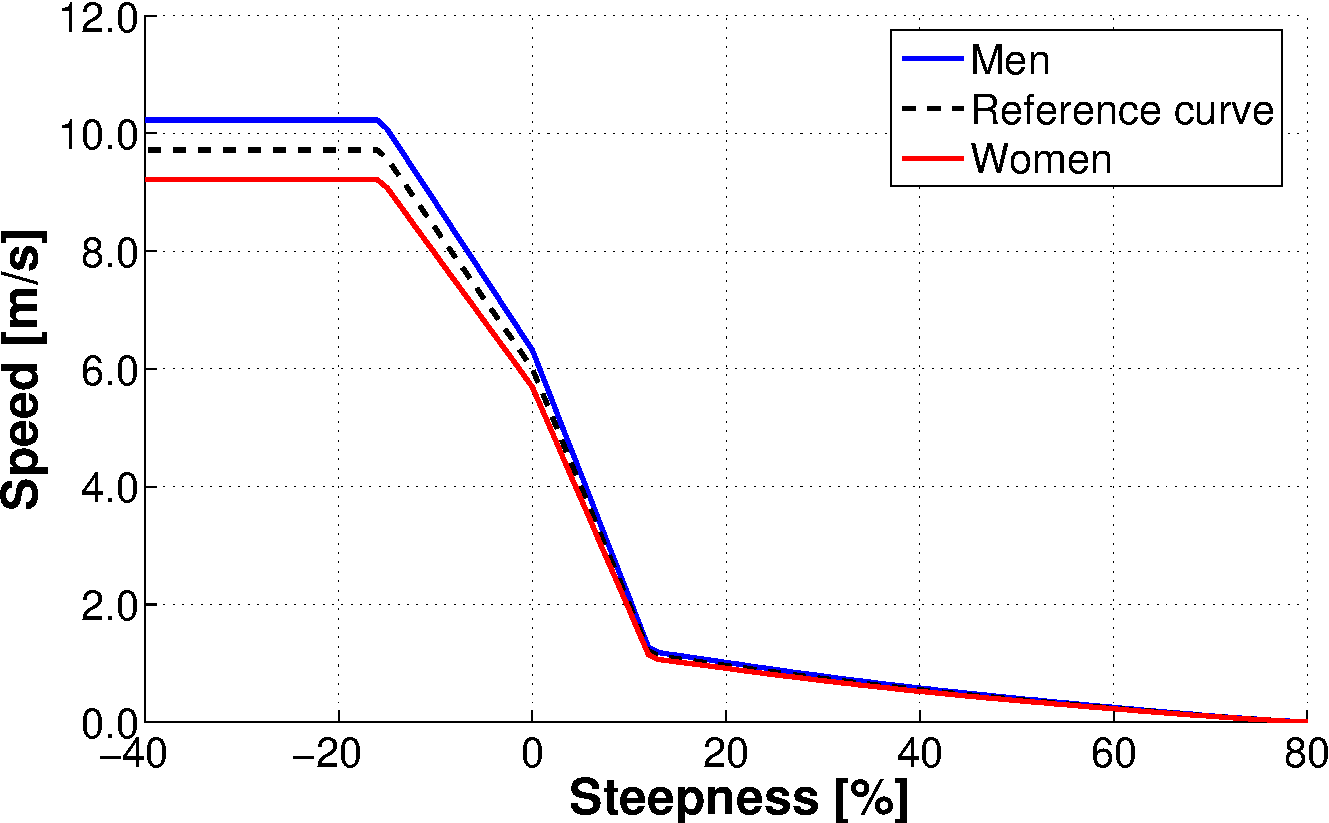
\includegraphics[width=0.70\textwidth, angle=0]{extending/figures/MultiModalSimulation/cyclistsSteepness}}%
  {\label{fig:labelCyclistsSteepness}}%
  {\vspace{4mm}}%

  \createsubfigure%
  {Age and steepness dependent speed}%
  {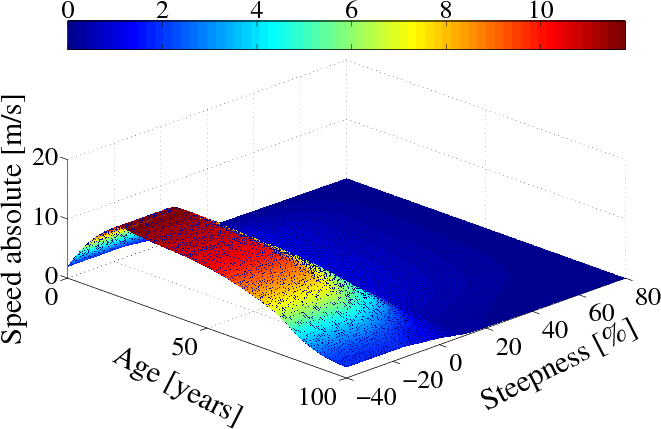
\includegraphics[width=0.70\textwidth, angle=0]{extending/figures/MultiModalSimulation/cyclists3d}}%
  {\label{fig:labelCyclistsAgeSteepness3d}}%
  {}%
}%
{}
%---------------------------------------------------------------------
\afterpage{\clearpage}	% force latex to place the figures somewhere near here and not at the end of the chapter

When calculating the steepness factor, it is distinguished whether a link goes uphill or downhill. When going uphill, the person's speed is reduced by a factor which is calculated based on the grade and a reference factor of 0.4002~m/s which is scaled by the same factor as the person's reference speed. I.e. the speed drop of slow people is lower than the drop of fast people. When the bike speed drops below the walk speed, which happens at a grade of approximately 12\%, it is assumed that the person's switches to walking (see Equation \ref{equ:bike_uphill}). For downhill links a reference factor of 0.2379~m/s is used. Additionally it is assumed that cyclists limit their speed to 35~km/h (9.7222 m/s; see Equation \ref{equ:bike_downhill}).

% default seems to be ~14.0
{\fontsize{12.8pt}{12}
\begin{align}
    v\textsubscript{person, bike} &= v\textsubscript{reference, bike} \cdot f\textsubscript{person}\\
    v\textsubscript{person, uphill} &= \text{max}
    \begin{cases}
        v\textsubscript{person, bike, flat} - 0.4002 \cdot |\text{grade}| \cdot f\textsubscript{person}\\
        v\textsubscript{person, walk, uphill}
    \end{cases}\label{equ:bike_uphill}\\
    v_{\textsubscript{person, downhill}} &= \text{min}
    \begin{cases}
        v\textsubscript{person, bike, flat} + 0.2379 \cdot |\text{grade}| \cdot f\textsubscript{person}\\
        9.7222
    \end{cases}\label{equ:bike_downhill}
\end{align}
}%

Another parameter that affects the speed of pedestrians and cyclists is the crowdedness of the link where they are physically present. Data to take this effect into account is again presented by \citet{Weidmann_TechRep_IVT_1992}. However, to calculate the crowdedness of a link, its geometry has to be taken into account. A method of doing this is e.g.~discussed by \citet{Laemmel_PhDThesis_2011}. 

% ##################################################################################################################
\section{Scenario}
The capabilities of the simulation extension for non-motorized traffic are demonstrated and validated using the scenario shown in Figure \ref{fig:MultiModalDemo}. Agents have to travel from house A to house B. They can go by car using route~1 or walk using route~2. The length of route 1 is chosen so that the free flow travel time equals the walk travel time of an average 50 year old man using route~2. Agents can choose whether they take route~1 or 2. While the walk travel time only depends on an agent's age, the car travel time depends on the number of agents also choosing route~1. Since the implementations of walk and bike mode differ only by the shape of the speed profiles, the conducted experiments are not performed a second time using bike instead of walk as non-car mode.

%---------------------------------------------------------------------
\createfigure%
{Multi-modal link extension}%
{Multi-modal link extension}%
{\label{fig:MultiModalDemo}}%
{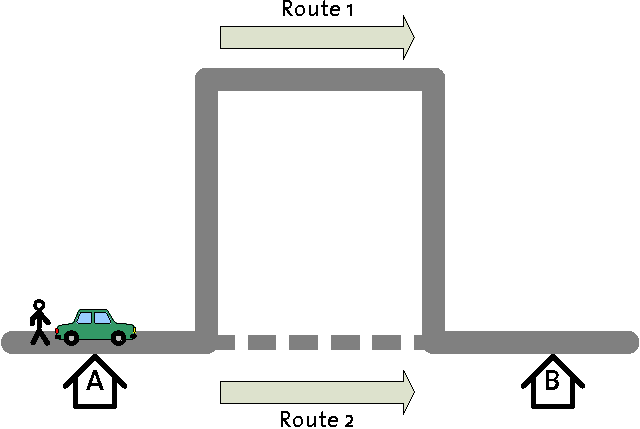
\includegraphics[width=0.75\textwidth, angle=0]{extending/figures/MultiModalSimulation/MultiModalDemo}}%
{}
%---------------------------------------------------------------------


To test the implementation, three parameters are varied. A first one is statisical spreading which is either enabled or disabled when calculating a person's speed. The transport mode which the agents use initially is a second parameter. The three settings used are \textit{100\% car}, \textit{random selection (i.e.\ 50\% car and 50\% walk)} and \textit{100\% walk}. Further, the capacity of route~1 is reduced. As a results, agents using that route might switch to route~2 since walking might be faster than beeing stuck in the resulting traffic jam. 

For each tested parameter combination, a simulation run with 100 iterations is performed. The simulated population contains 10'000 agents. For each agent, random values for their age (between 18 and 100), gender and depature time between 08:00 and 12:00 are selected.

%---------------------------------------------------------------------
\subsection{Statisical Spreading}
In a first set of experiments, the influence of statistical spreading on persons' walk speed is tested. Persons' initial transport modes are chosen randomly. Results are shown in Figures \ref{fig:statisticalSpreadingAvgCarTravelTimes} to \ref{fig:statisticalSpreadingMaleAndFemale}. The average walk and car travel times for different capacities of route~1 are compared in Figures \ref{fig:statisticalSpreadingAvgCarTravelTimes} and \ref{fig:statisticalSpreadingAvgWalkTravelTimes}. As can be seen, the average values are hardly affected. The number of performed walk respectively car trips  for different capacities is compared in Figures \ref{fig:statisticalSpreadingNumCarTrips} and \ref{fig:statisticalSpreadingNumWalkTrips}. Again, hardly any difference can be seen. This indicates that adding statistical spreading to the persons' walk speed does not shift the population's average walk speed.

\ah{Resultate stark komprimieren!}

%---------------------------------------------------------------------
\createfigure%
{Influence of statistical spreading -- Average car travel times}%
{Influence of statistical spreading -- Average car travel times}%
{\label{fig:statisticalSpreadingAvgCarTravelTimes}}%
{%
  \createsubfigure%
  {Capacity 500 veh/h}%
  {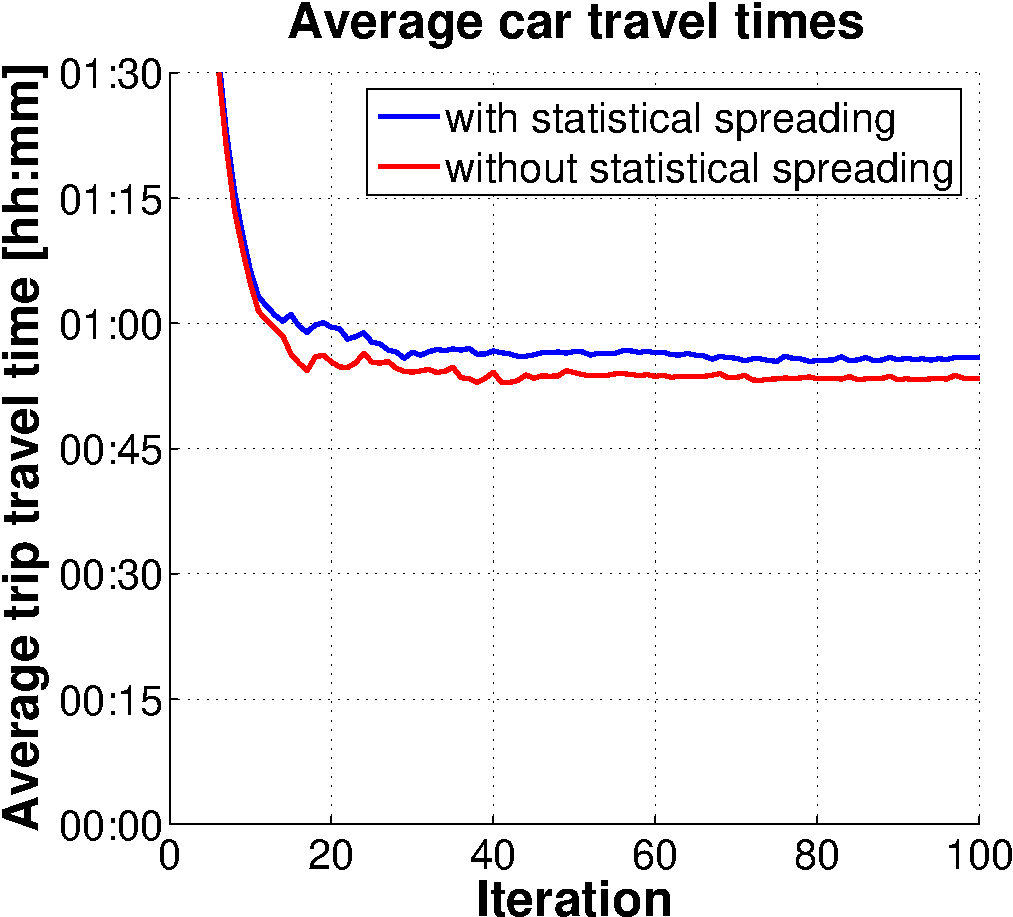
\includegraphics[width=0.47\textwidth, angle=0, trim=0mm 0mm 0mm 9mm, clip=true]{extending/figures/MultiModalSimulation/simulations/avg_car_traveltime_scatter_500}}%
  {\label{}}%
  {\hspace{3mm}}%
  \createsubfigure%
  {Capacity 1000 veh/h}%
  {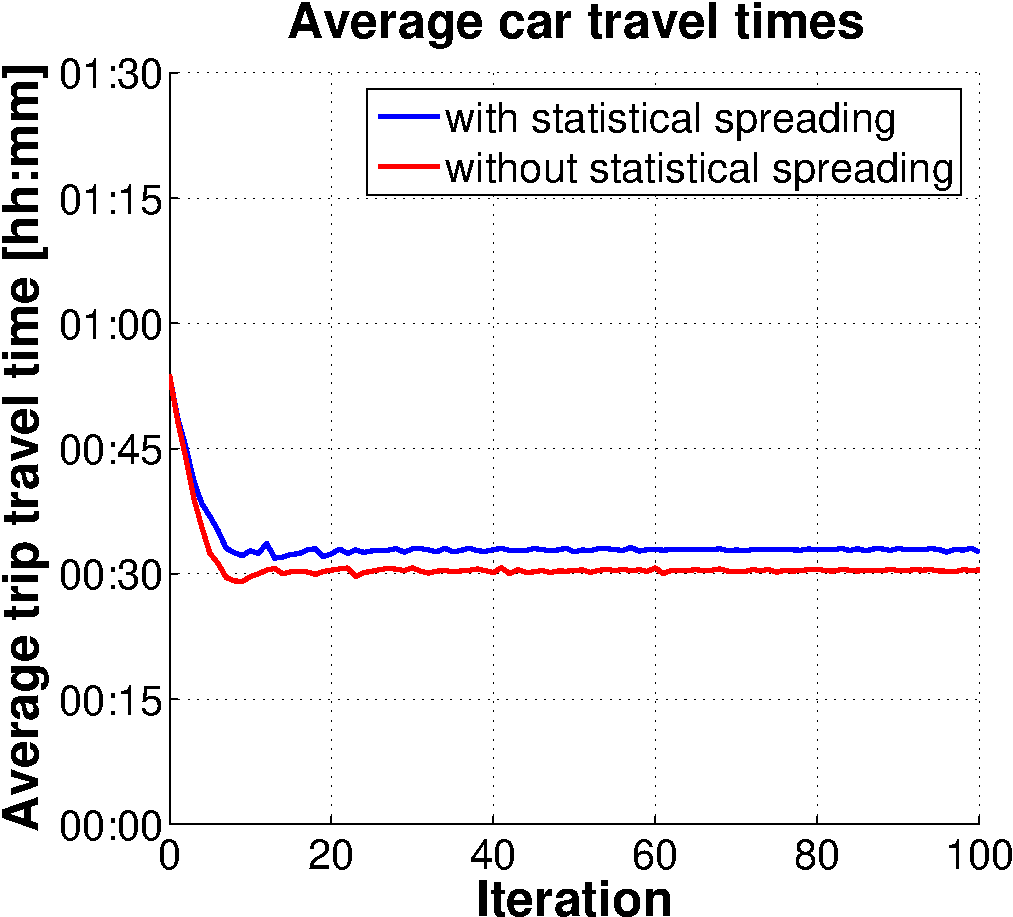
\includegraphics[width=0.47\textwidth, angle=0, trim=0mm 0mm 0mm 9mm, clip=true]{extending/figures/MultiModalSimulation/simulations/avg_car_traveltime_scatter_1000}}%
  {\label{}}%
  {\vspace{7.5mm}}%

  \createsubfigure%
  {Capacity 1500 veh/h}%
  {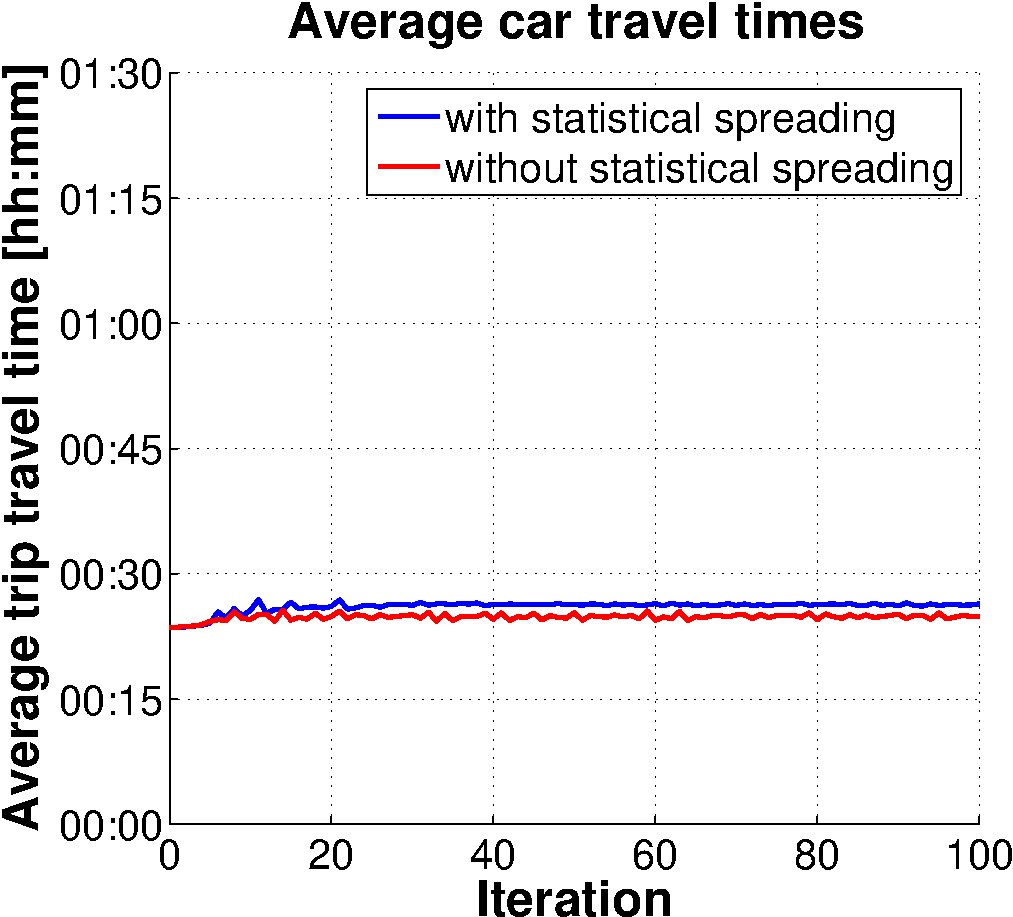
\includegraphics[width=0.47\textwidth, angle=0, trim=0mm 0mm 0mm 9mm, clip=true]{extending/figures/MultiModalSimulation/simulations/avg_car_traveltime_scatter_1500}}%
  {\label{}}%
  {\hspace{3mm}}%
  \createsubfigure%
  {Capacity 2000 veh/h}%
  {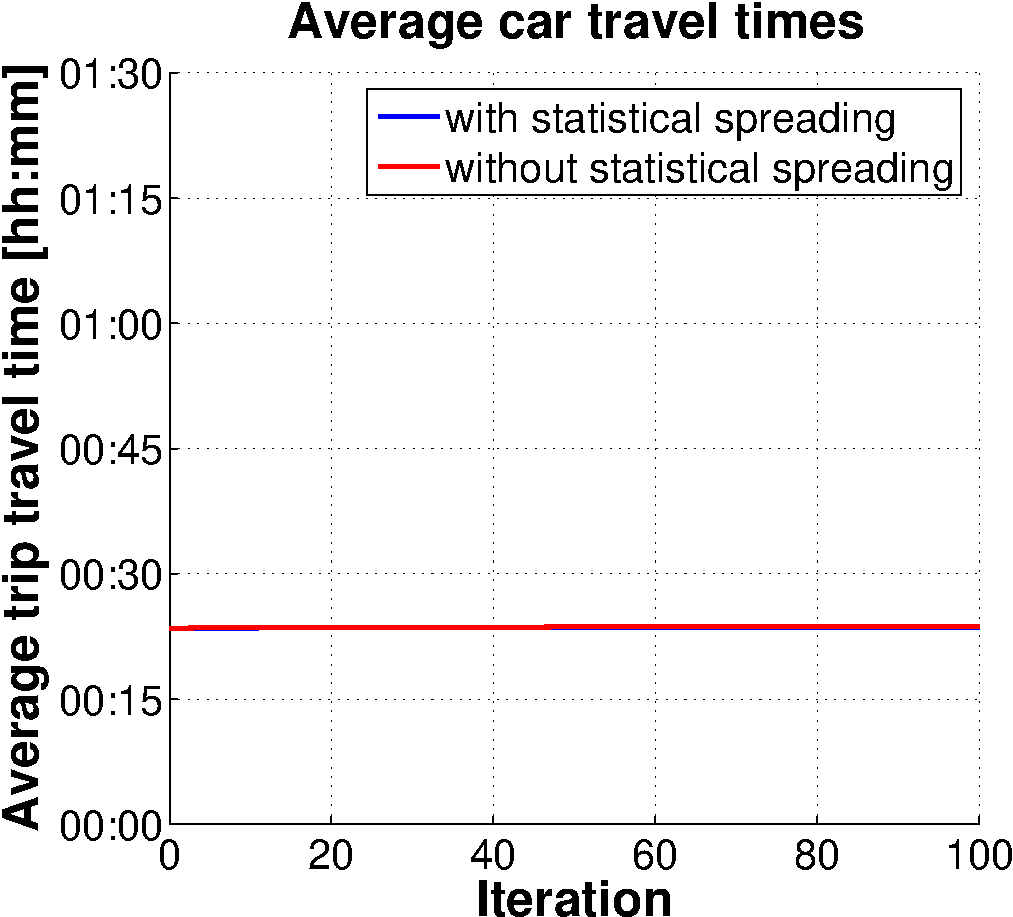
\includegraphics[width=0.47\textwidth, angle=0, trim=0mm 0mm 0mm 9mm, clip=true]{extending/figures/MultiModalSimulation/simulations/avg_car_traveltime_scatter_2000}}%
  {\label{}}%
  {\vspace{7.5mm}}%

  \createsubfigure%
  {Capacity 2500 veh/h}%
  {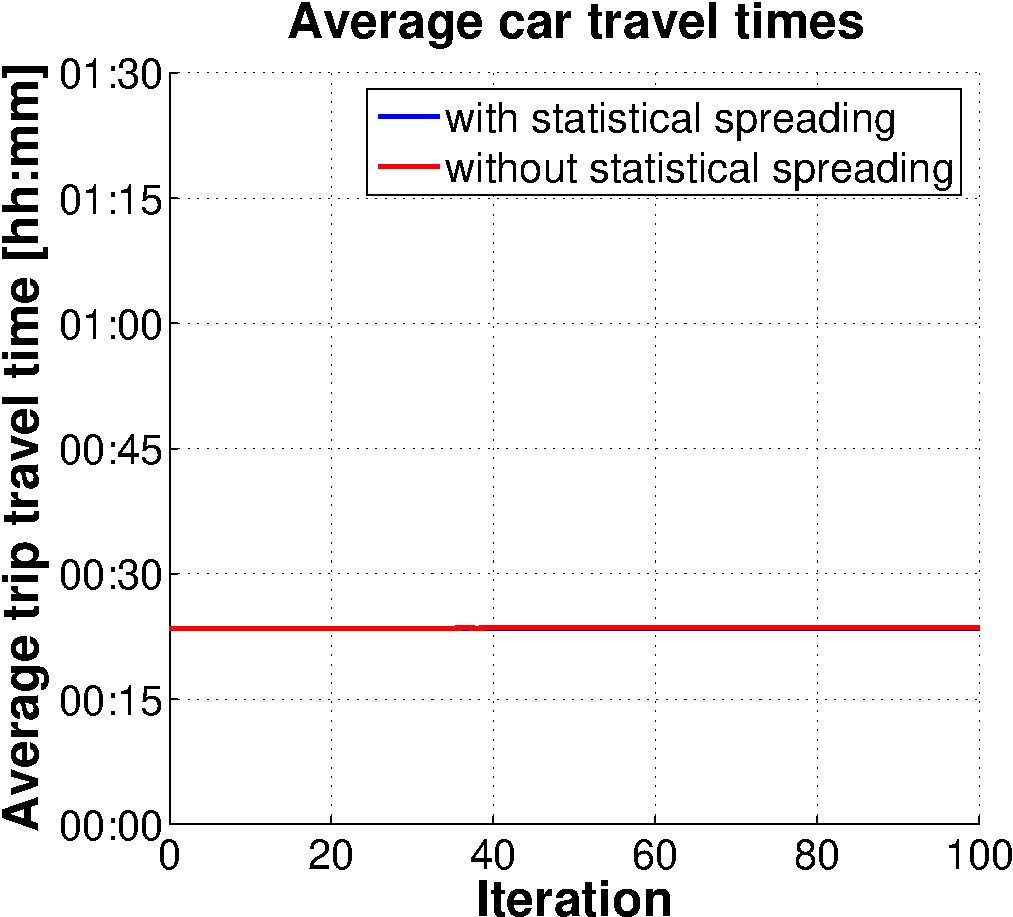
\includegraphics[width=0.47\textwidth, angle=0, trim=0mm 0mm 0mm 9mm, clip=true]{extending/figures/MultiModalSimulation/simulations/avg_car_traveltime_scatter_2500}}%
  {\label{}}%
  {\hspace{3mm}}%
  \createsubfigure%
  {Capacity unlimited}%
  {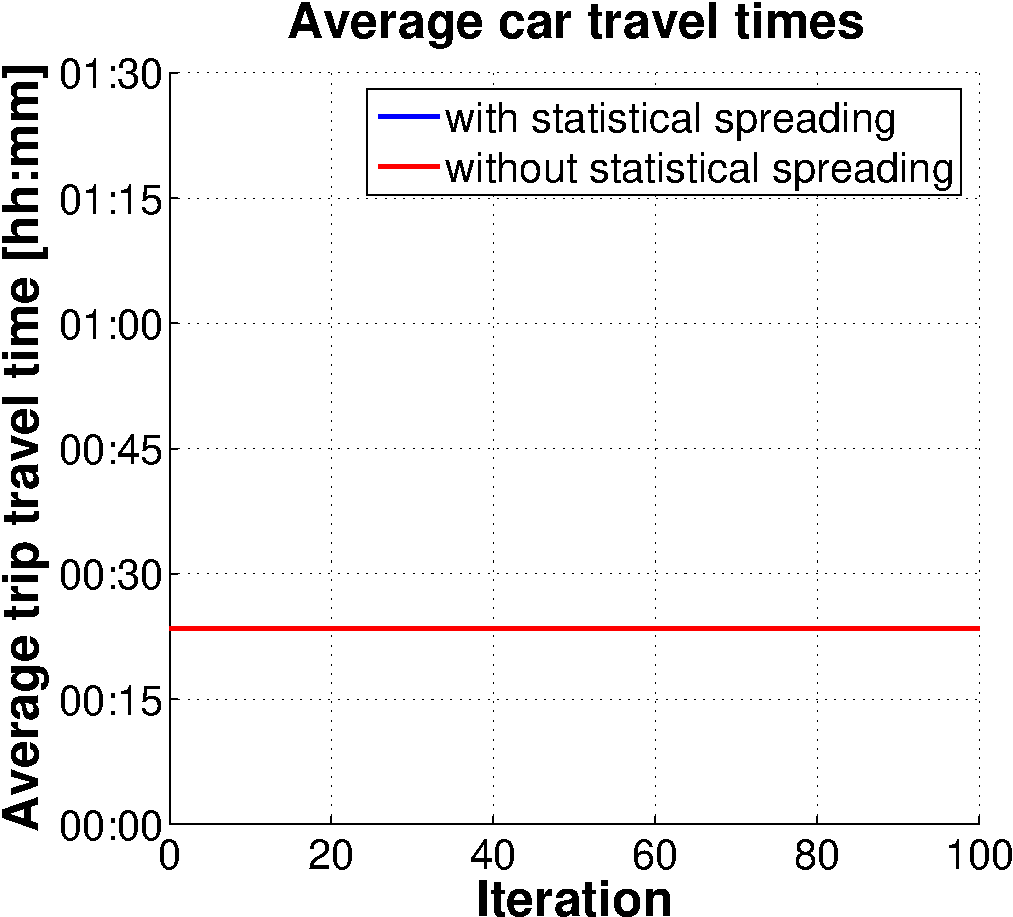
\includegraphics[width=0.47\textwidth, angle=0, trim=0mm 0mm 0mm 9mm, clip=true]{extending/figures/MultiModalSimulation/simulations/avg_car_traveltime_scatter_unlimited}}%
  {\label{}}%
  {}%
}%
{}
%---------------------------------------------------------------------

%---------------------------------------------------------------------
\createfigure%
{Influence of statistical spreading -- Average walk travel times}%
{Influence of statistical spreading -- Average walk travel times}%
{\label{fig:statisticalSpreadingAvgWalkTravelTimes}}%
{%
  \createsubfigure%
  {Capacity 500 veh/h}%
  {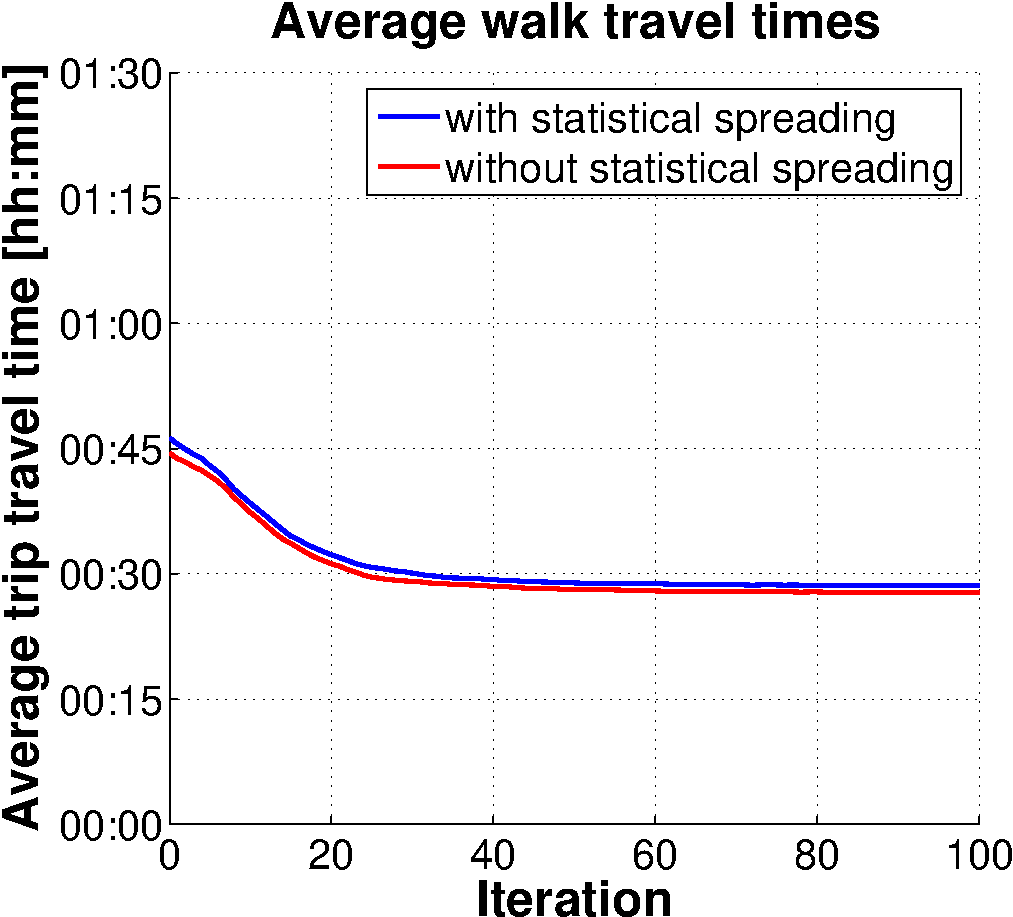
\includegraphics[width=0.47\textwidth, angle=0, trim=0mm 0mm 0mm 9mm, clip=true]{extending/figures/MultiModalSimulation/simulations/avg_walk_traveltime_scatter_500}}%
  {\label{}}%
  {\hspace{3mm}}%
  \createsubfigure%
  {Capacity 1000 veh/h}%
  {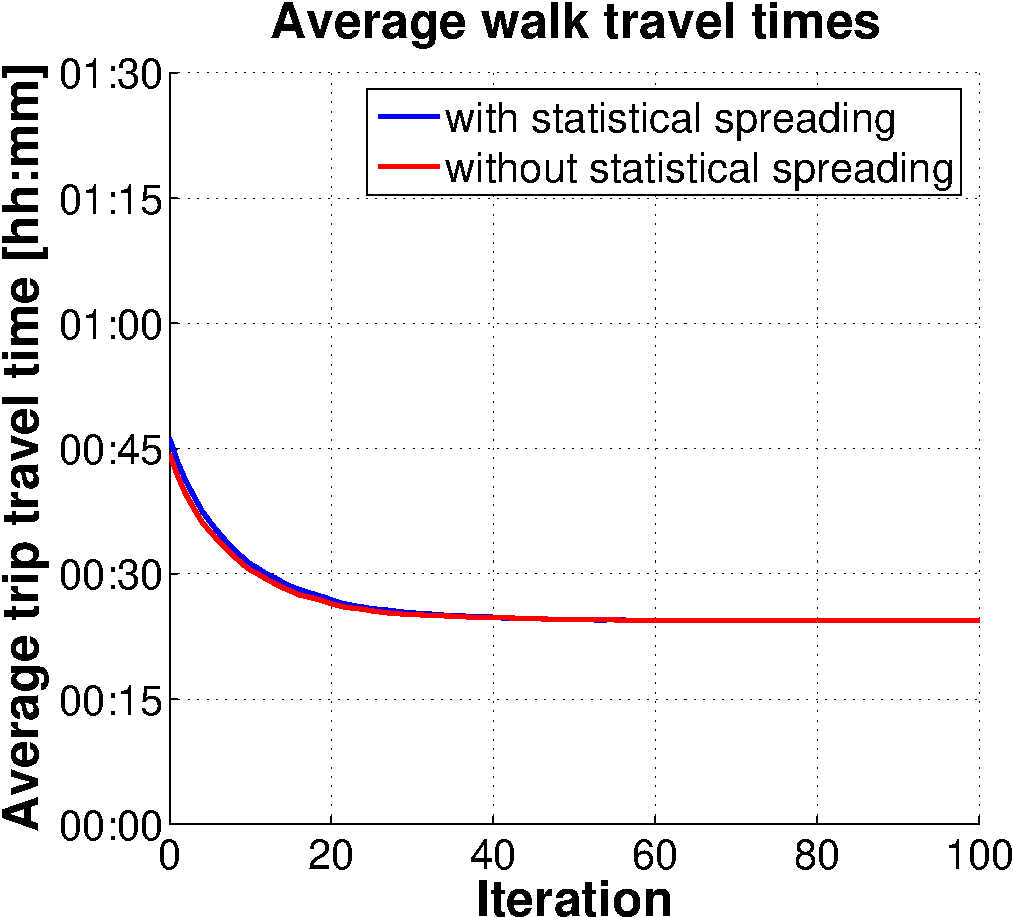
\includegraphics[width=0.47\textwidth, angle=0, trim=0mm 0mm 0mm 9mm, clip=true]{extending/figures/MultiModalSimulation/simulations/avg_walk_traveltime_scatter_1000}}%
  {\label{}}%
  {\vspace{7.5mm}}%

  \createsubfigure%
  {Capacity 1500 veh/h}%
  {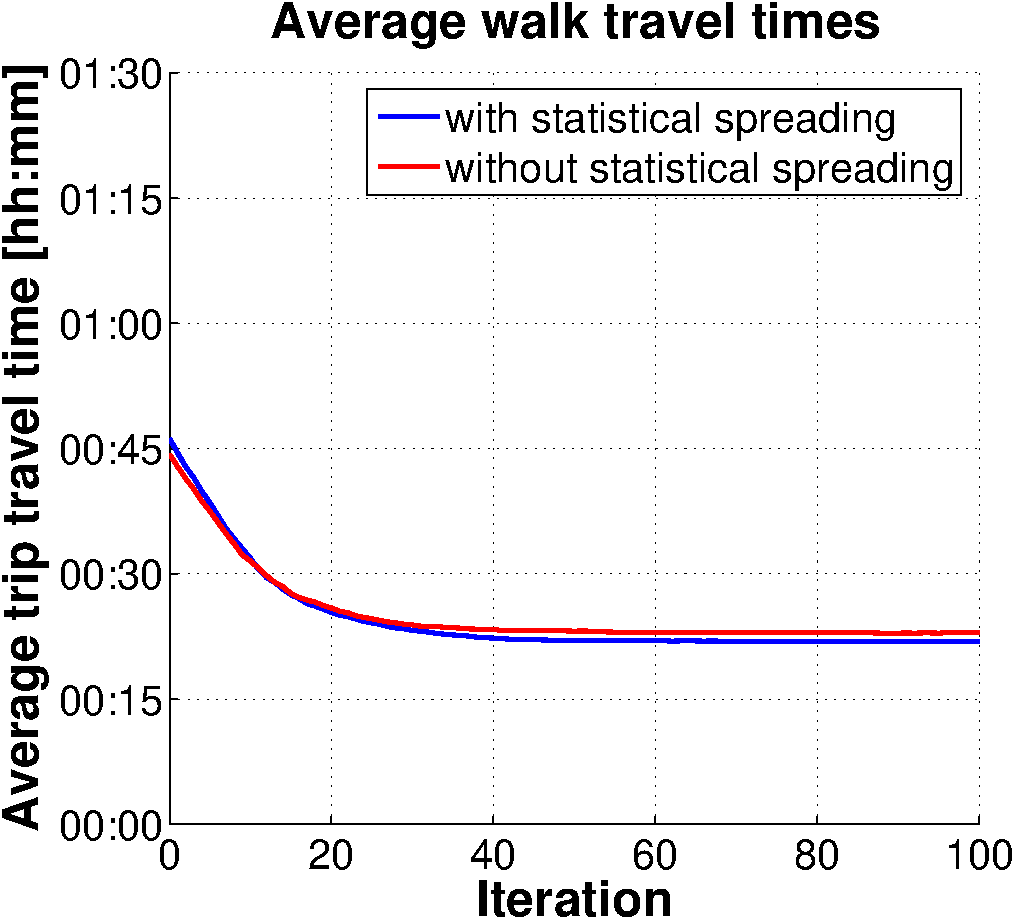
\includegraphics[width=0.47\textwidth, angle=0, trim=0mm 0mm 0mm 9mm, clip=true]{extending/figures/MultiModalSimulation/simulations/avg_walk_traveltime_scatter_1500}}%
  {\label{}}%
  {\hspace{3mm}}%
  \createsubfigure%
  {Capacity 2000 veh/h}%
  {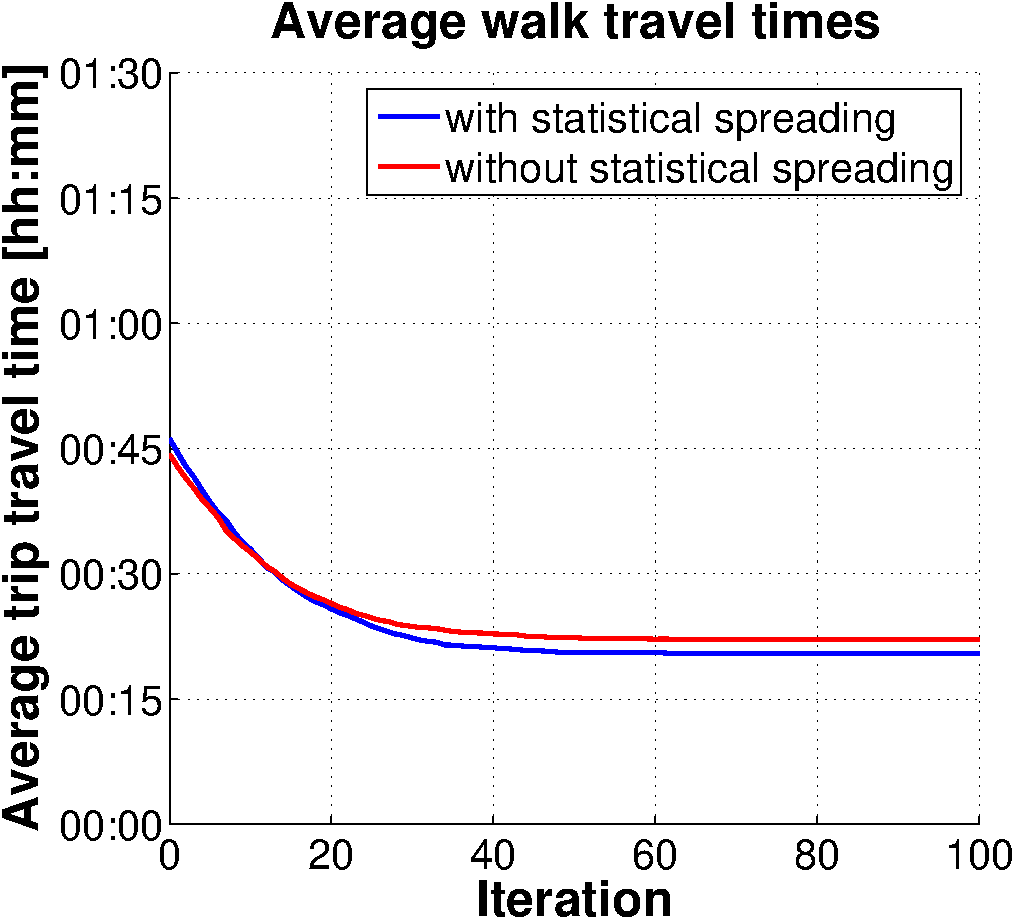
\includegraphics[width=0.47\textwidth, angle=0, trim=0mm 0mm 0mm 9mm, clip=true]{extending/figures/MultiModalSimulation/simulations/avg_walk_traveltime_scatter_2000}}%
  {\label{}}%
  {\vspace{7.5mm}}%

  \createsubfigure%
  {Capacity 2500 veh/h}%
  {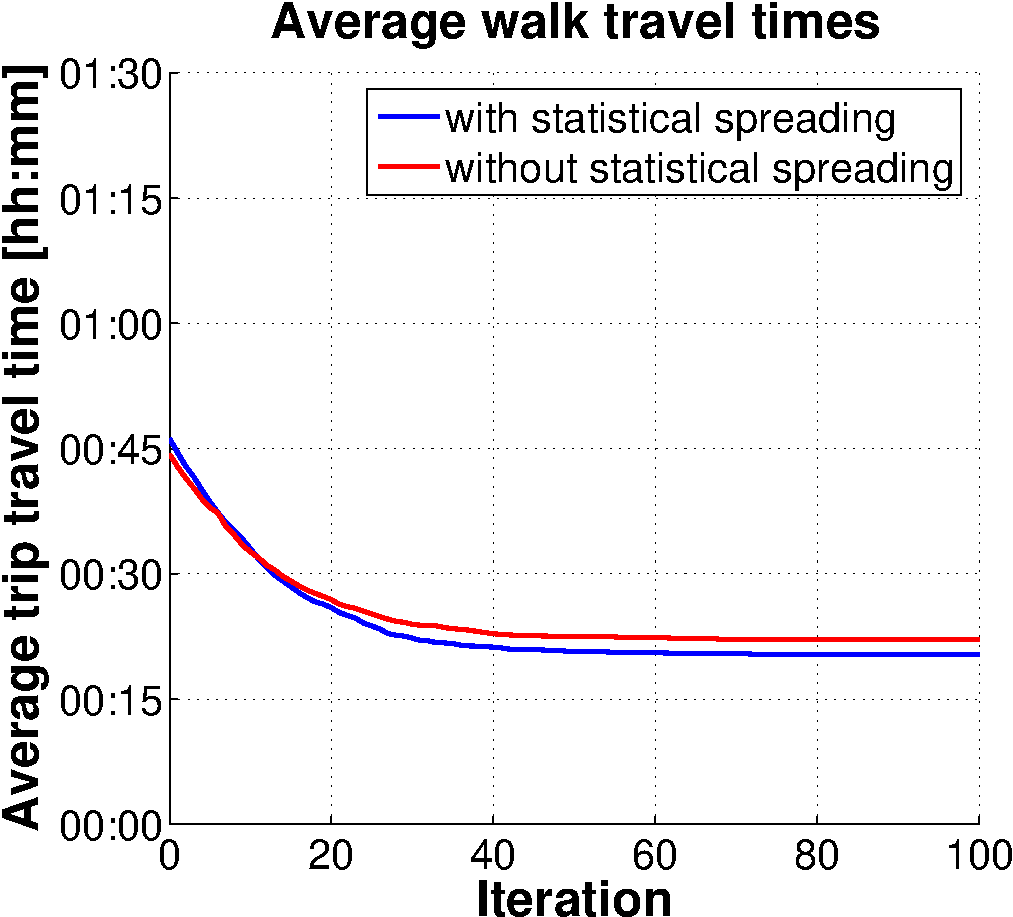
\includegraphics[width=0.47\textwidth, angle=0, trim=0mm 0mm 0mm 9mm, clip=true]{extending/figures/MultiModalSimulation/simulations/avg_walk_traveltime_scatter_2500}}%
  {\label{}}%
  {\hspace{3mm}}%
  \createsubfigure%
  {Capacity unlimited}%
  {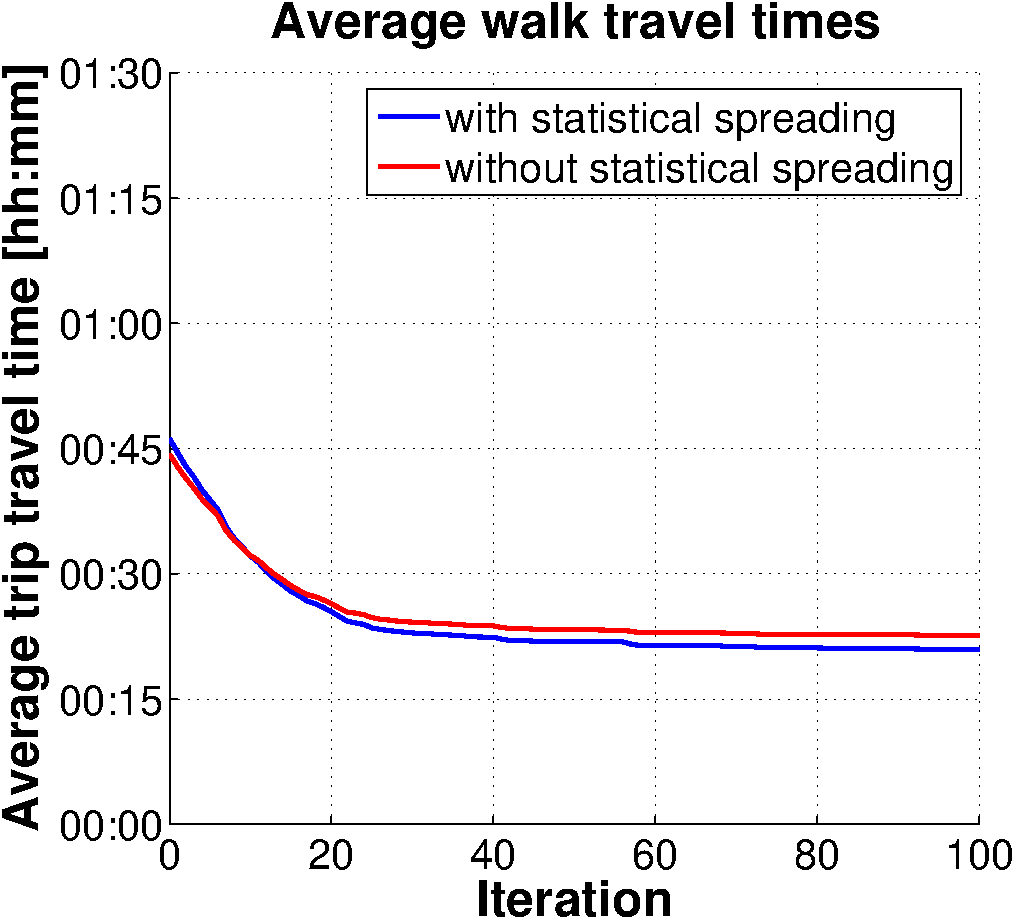
\includegraphics[width=0.47\textwidth, angle=0, trim=0mm 0mm 0mm 9mm, clip=true]{extending/figures/MultiModalSimulation/simulations/avg_walk_traveltime_scatter_unlimited}}%
  {\label{}}%
  {}%
}%
{}
%---------------------------------------------------------------------

%---------------------------------------------------------------------
\createfigure%
{Influence of statistical spreading -- Number of car trips}%
{Influence of statistical spreading -- Number of car trips}%
{\label{fig:statisticalSpreadingNumCarTrips}}%
{%
  \createsubfigure%
  {Capacity 500 veh/h}%
  {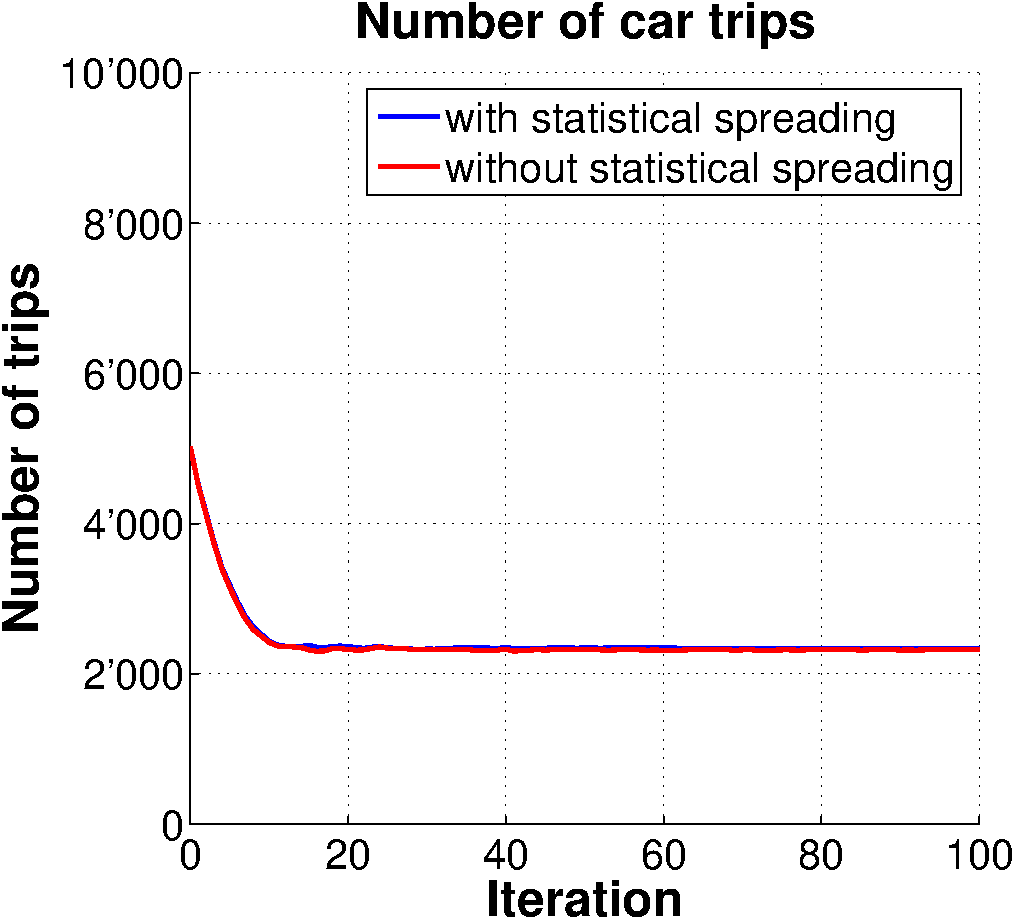
\includegraphics[width=0.47\textwidth, angle=0, trim=0mm 0mm 0mm 9mm, clip=true]{extending/figures/MultiModalSimulation/simulations/num_car_trips_no_scatter_500}}%
  {\label{}}%
  {\hspace{3mm}}%
  \createsubfigure%
  {Capacity 1000 veh/h}%
  {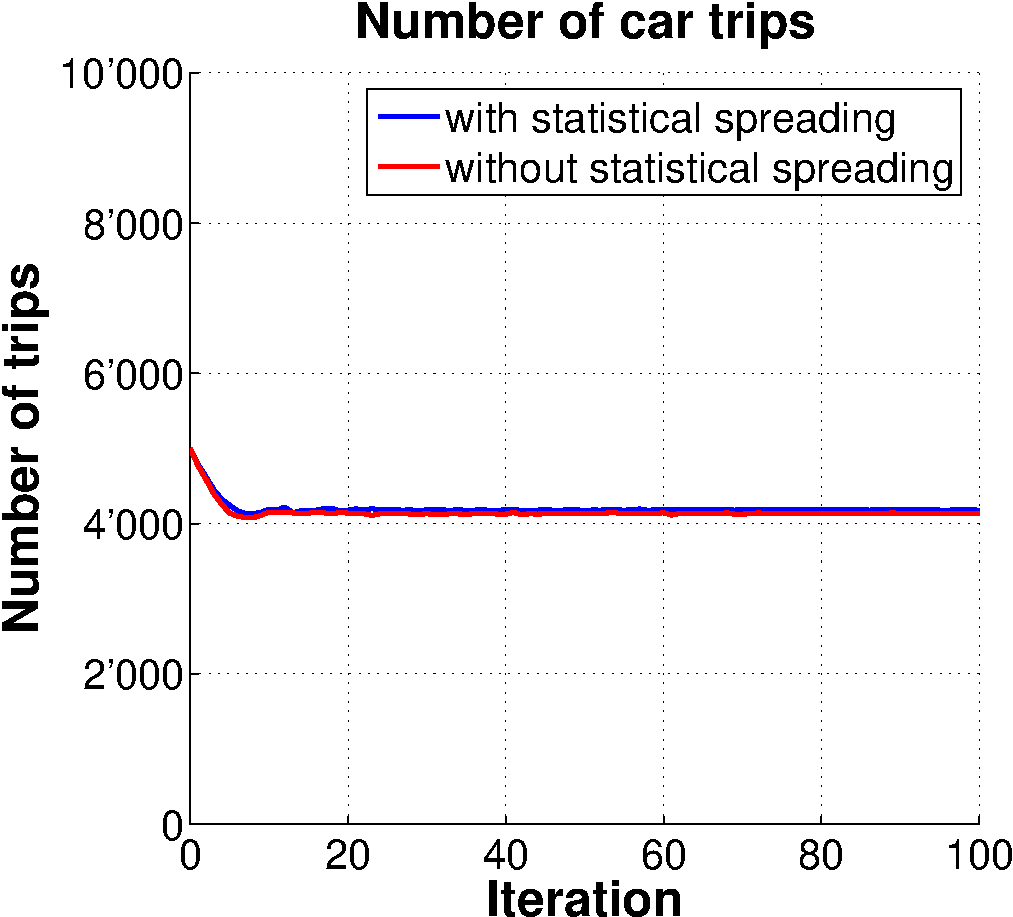
\includegraphics[width=0.47\textwidth, angle=0, trim=0mm 0mm 0mm 9mm, clip=true]{extending/figures/MultiModalSimulation/simulations/num_car_trips_no_scatter_1000}}%
  {\label{}}%
  {\vspace{7.5mm}}%

  \createsubfigure%
  {Capacity 1500 veh/h}%
  {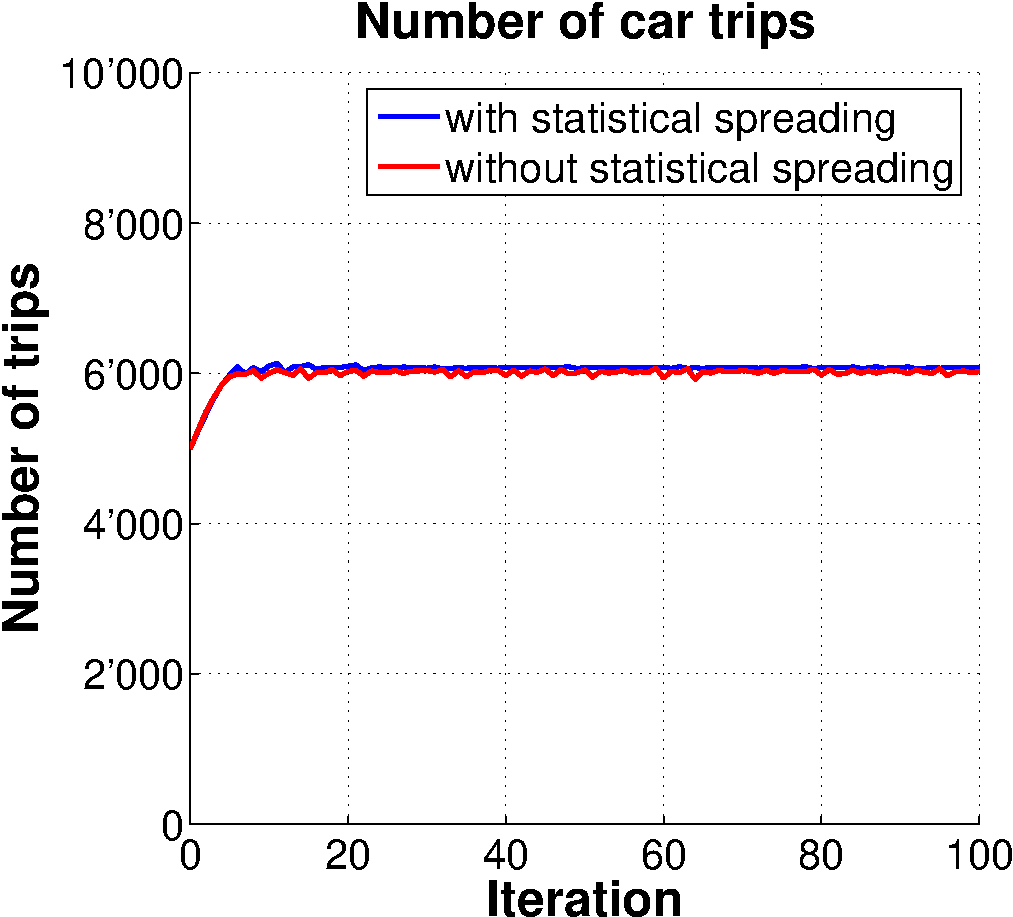
\includegraphics[width=0.47\textwidth, angle=0, trim=0mm 0mm 0mm 9mm, clip=true]{extending/figures/MultiModalSimulation/simulations/num_car_trips_no_scatter_1500}}%
  {\label{}}%
  {\hspace{3mm}}%
  \createsubfigure%
  {Capacity 2000 veh/h}%
  {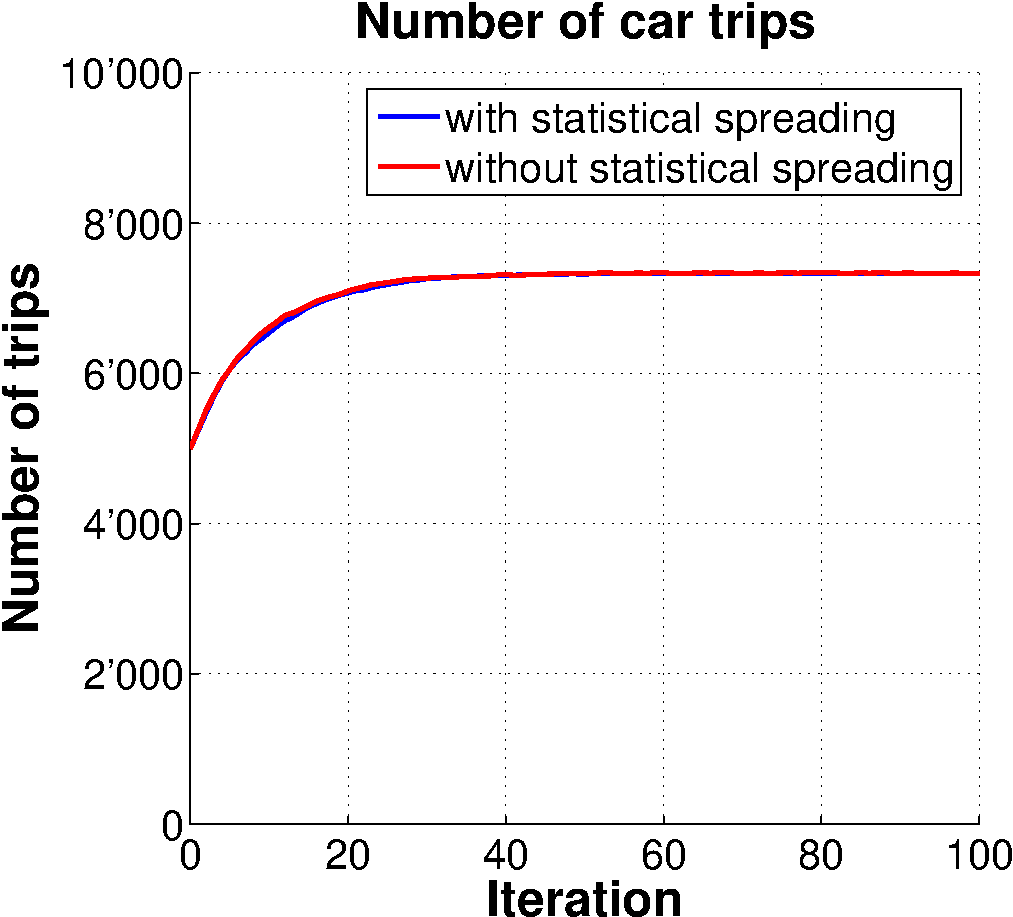
\includegraphics[width=0.47\textwidth, angle=0, trim=0mm 0mm 0mm 9mm, clip=true]{extending/figures/MultiModalSimulation/simulations/num_car_trips_no_scatter_2000}}%
  {\label{}}%
  {\vspace{7.5mm}}%

  \createsubfigure%
  {Capacity 2500 veh/h}%
  {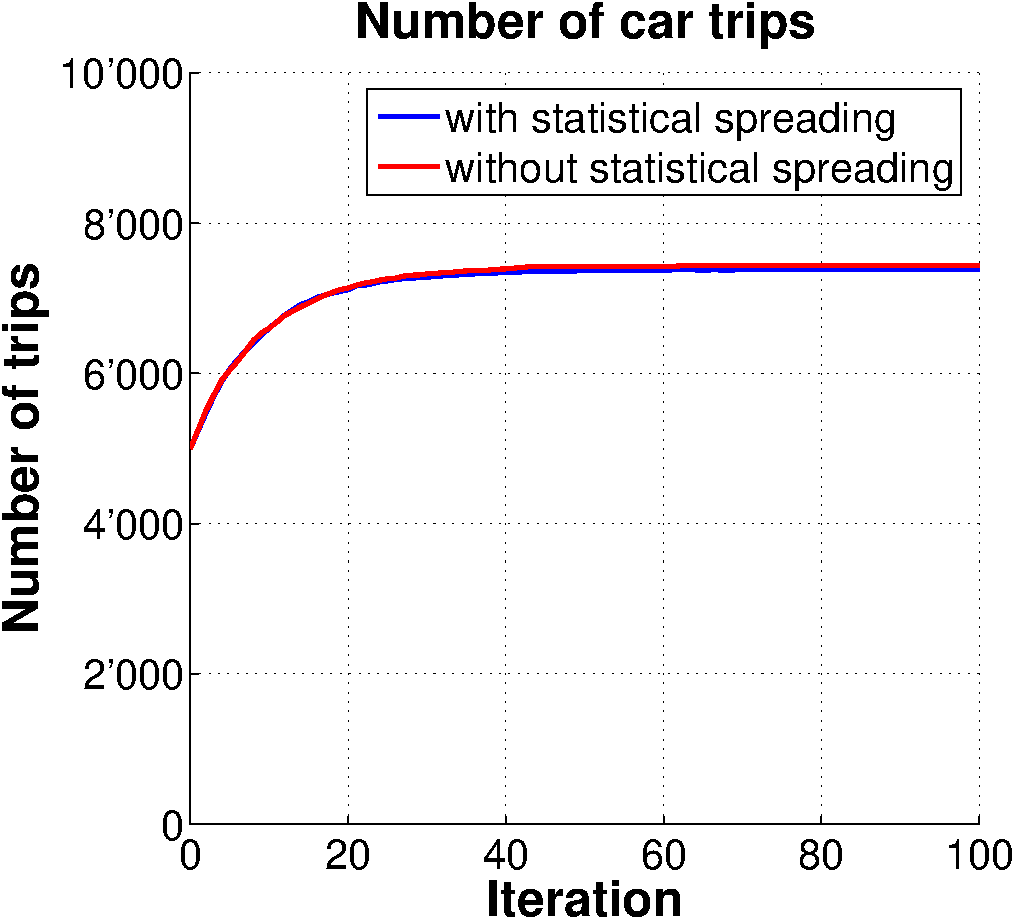
\includegraphics[width=0.47\textwidth, angle=0, trim=0mm 0mm 0mm 9mm, clip=true]{extending/figures/MultiModalSimulation/simulations/num_car_trips_no_scatter_2500}}%
  {\label{}}%
  {\hspace{3mm}}%
  \createsubfigure%
  {Capacity unlimited}%
  {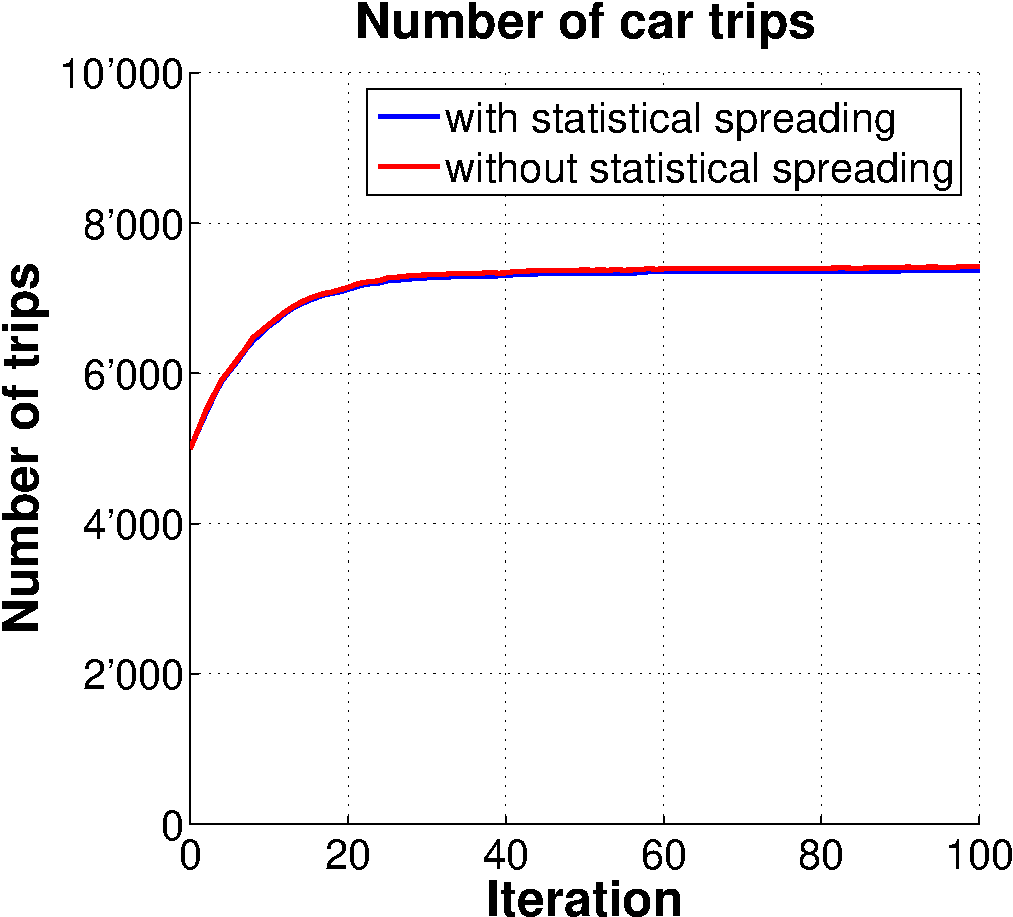
\includegraphics[width=0.47\textwidth, angle=0, trim=0mm 0mm 0mm 9mm, clip=true]{extending/figures/MultiModalSimulation/simulations/num_car_trips_no_scatter_unlimited}}%
  {\label{}}%
  {}%
}%
{}
%---------------------------------------------------------------------

%---------------------------------------------------------------------
\createfigure%
{Influence of statistical spreading -- Number of walk trips}%
{Influence of statistical spreading -- Number of walk trips}%
{\label{fig:statisticalSpreadingNumWalkTrips}}%
{%
  \createsubfigure%
  {Capacity 500 veh/h}%
  {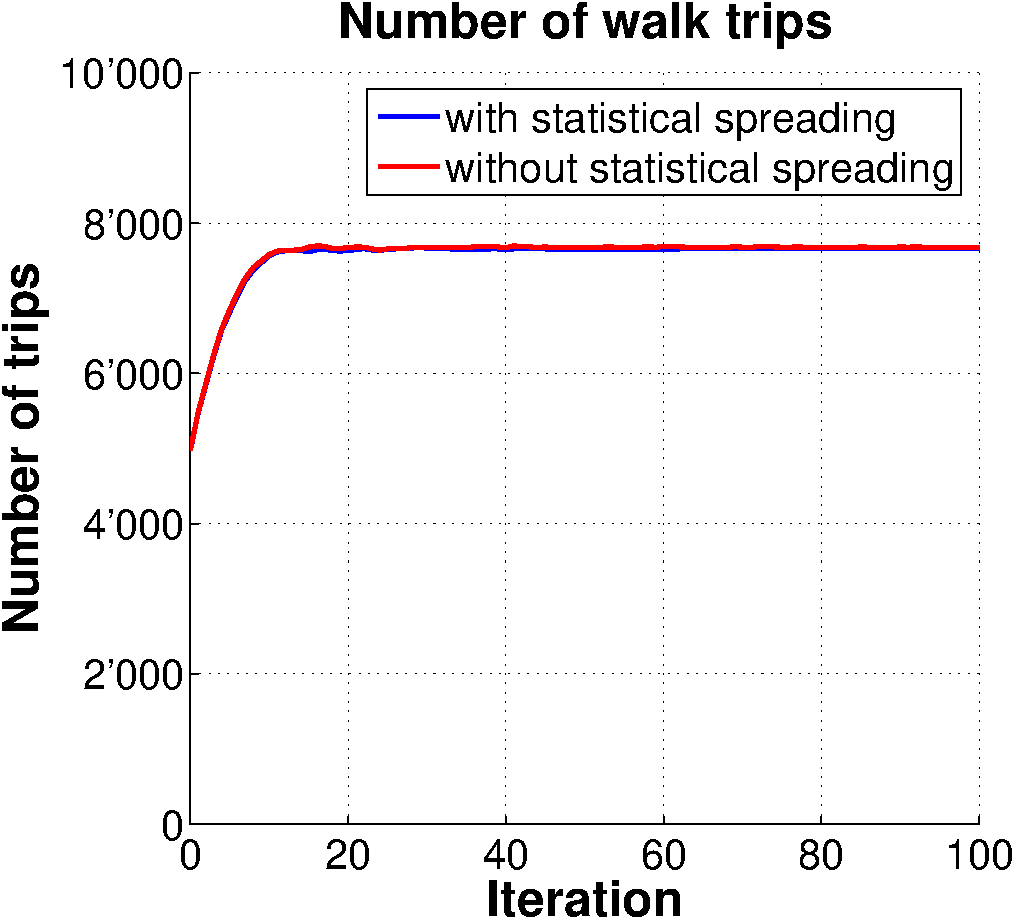
\includegraphics[width=0.47\textwidth, angle=0, trim=0mm 0mm 0mm 9mm, clip=true]{extending/figures/MultiModalSimulation/simulations/num_walk_trips_no_scatter_500}}%
  {\label{}}%
  {\hspace{3mm}}%
  \createsubfigure%
  {Capacity 1000 veh/h}%
  {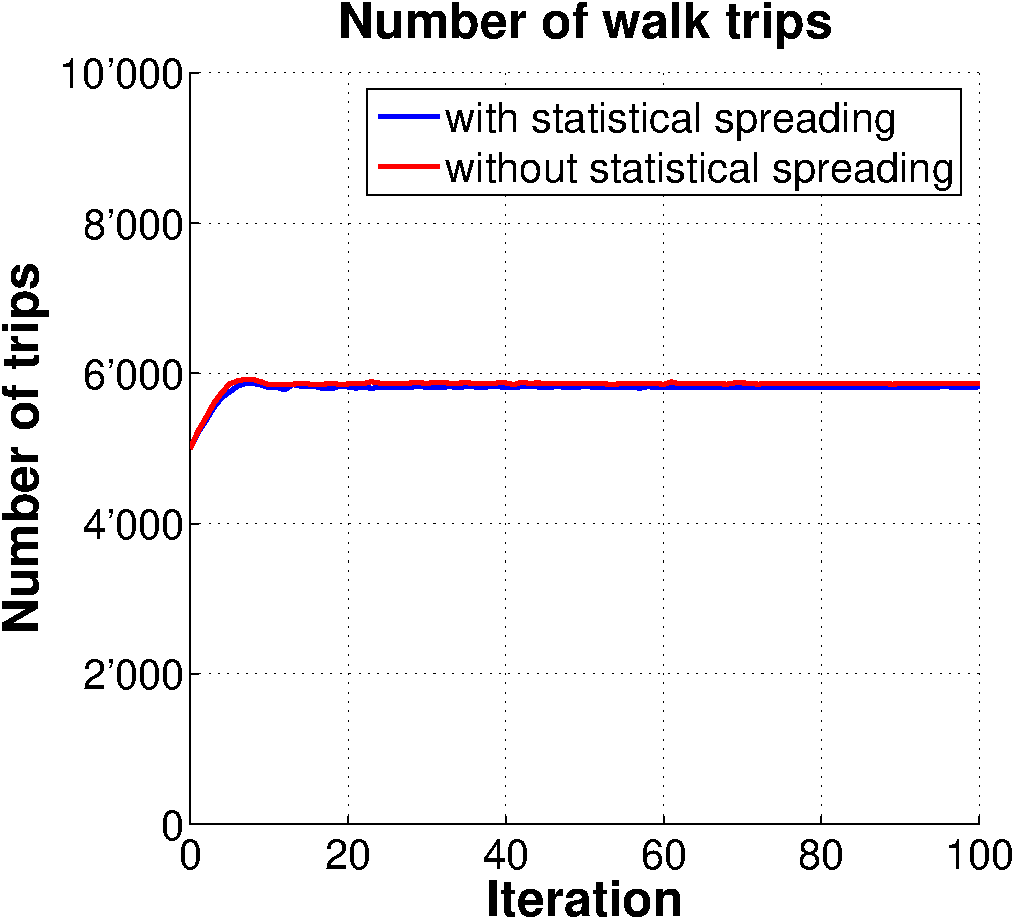
\includegraphics[width=0.47\textwidth, angle=0, trim=0mm 0mm 0mm 9mm, clip=true]{extending/figures/MultiModalSimulation/simulations/num_walk_trips_no_scatter_1000}}%
  {\label{}}%
  {\vspace{7.5mm}}%

  \createsubfigure%
  {Capacity 1500 veh/h}%
  {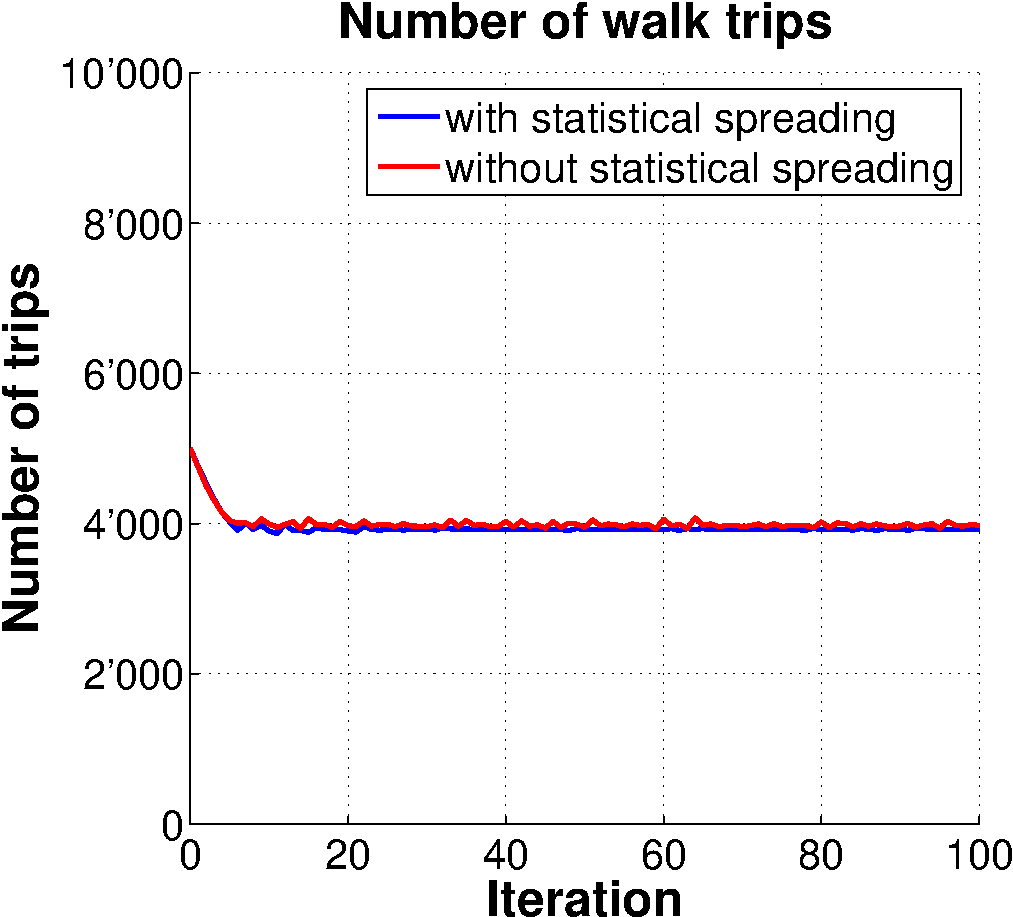
\includegraphics[width=0.47\textwidth, angle=0, trim=0mm 0mm 0mm 9mm, clip=true]{extending/figures/MultiModalSimulation/simulations/num_walk_trips_no_scatter_1500}}%
  {\label{}}%
  {\hspace{3mm}}%
  \createsubfigure%
  {Capacity 2000 veh/h}%
  {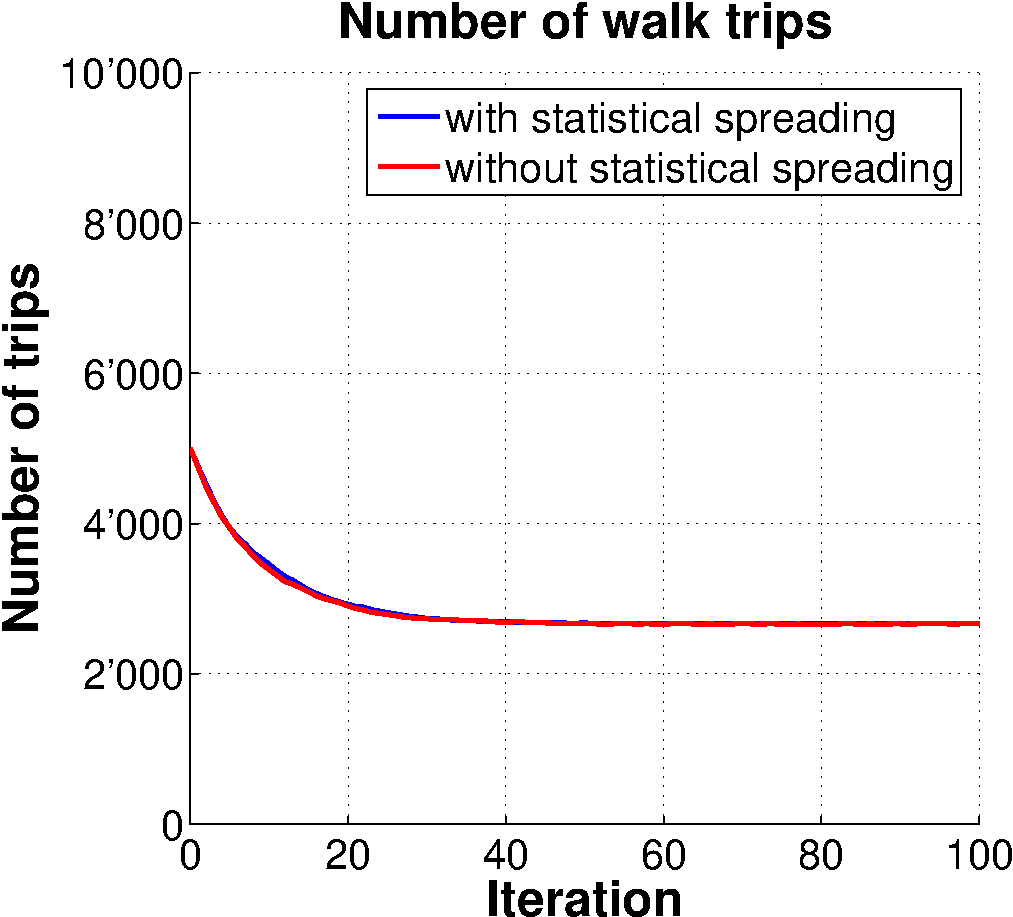
\includegraphics[width=0.47\textwidth, angle=0, trim=0mm 0mm 0mm 9mm, clip=true]{extending/figures/MultiModalSimulation/simulations/num_walk_trips_no_scatter_2000}}%
  {\label{}}%
  {\vspace{7.5mm}}%

  \createsubfigure%
  {Capacity 2500 veh/h}%
  {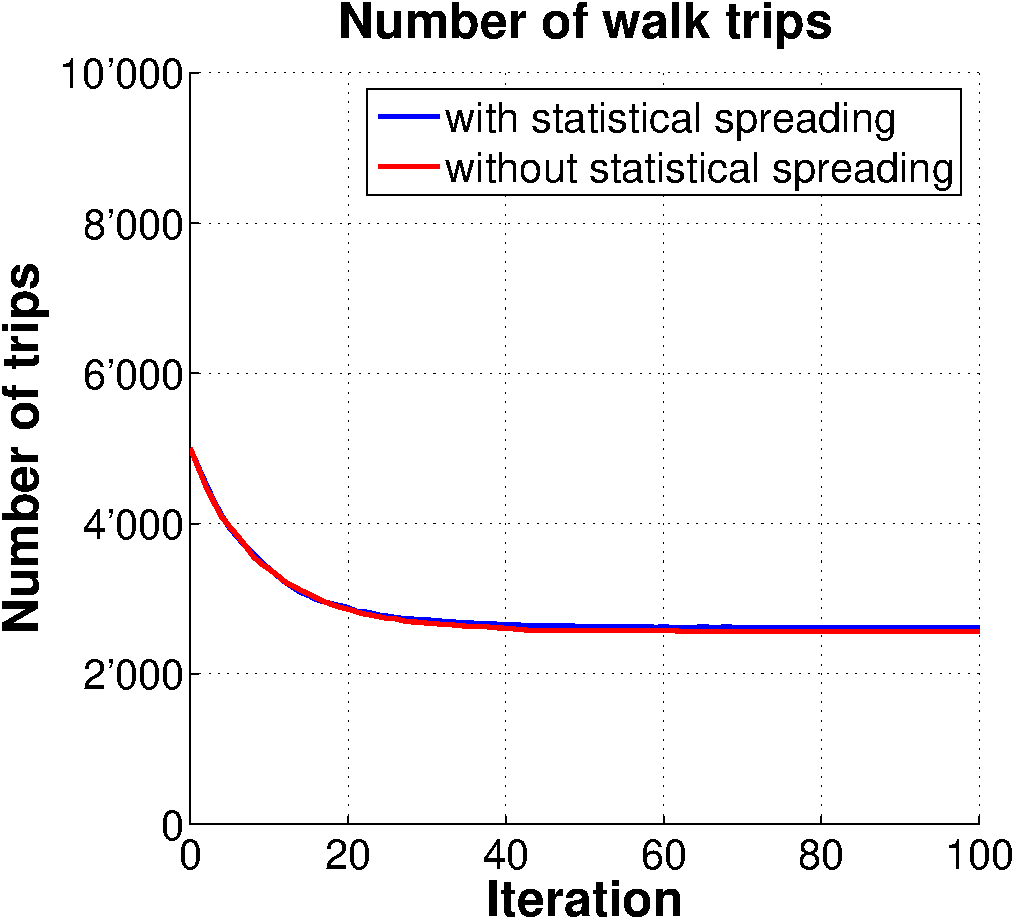
\includegraphics[width=0.47\textwidth, angle=0, trim=0mm 0mm 0mm 9mm, clip=true]{extending/figures/MultiModalSimulation/simulations/num_walk_trips_no_scatter_2500}}%
  {\label{}}%
  {\hspace{3mm}}%
  \createsubfigure%
  {Capacity unlimited}%
  {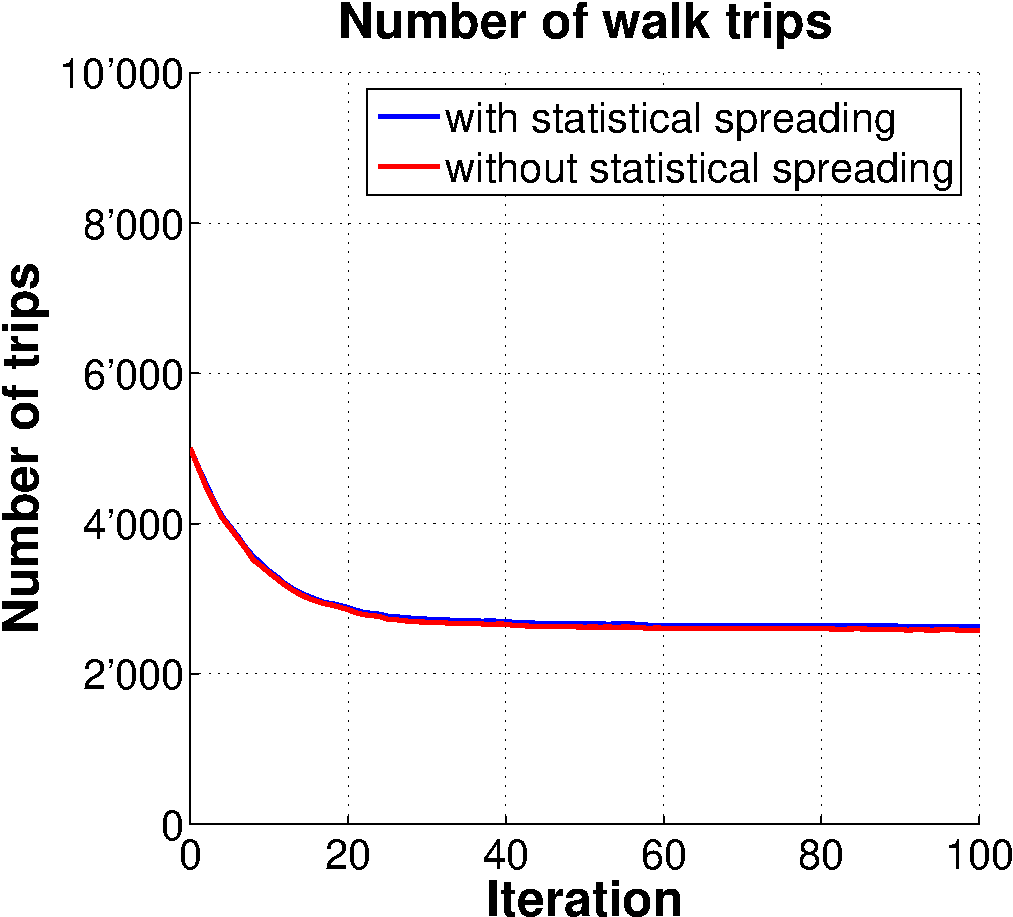
\includegraphics[width=0.45\textwidth, angle=0, trim=0mm 0mm 0mm 9mm, clip=true]{extending/figures/MultiModalSimulation/simulations/num_walk_trips_no_scatter_unlimited}}%
  {\label{}}%
  {}%
}%
{}
%---------------------------------------------------------------------

% moved this to a place after the figures...
%Figures \ref{fig:statisticalSpreadingAgeDistribution} and \ref{fig:statisticalSpreadingAgeDistributionWithSpreading} show the age distribution---separated into male and female---of all agents chose walking. As expected, the lower the capacity of route~1, the more agents prefer walking over going by car. The results indicate that enabling statistical spreading broadens and flattens the distribution significantly. 

%---------------------------------------------------------------------
\createfigure%
{Influence of statistical spreading -- Age distribution without spreading}%
{Influence of statistical spreading -- Age distribution without spreading}%
{\label{fig:statisticalSpreadingAgeDistribution}}%
{%
  \createsubfigure%
  {Capacity 500 veh/h}%
  {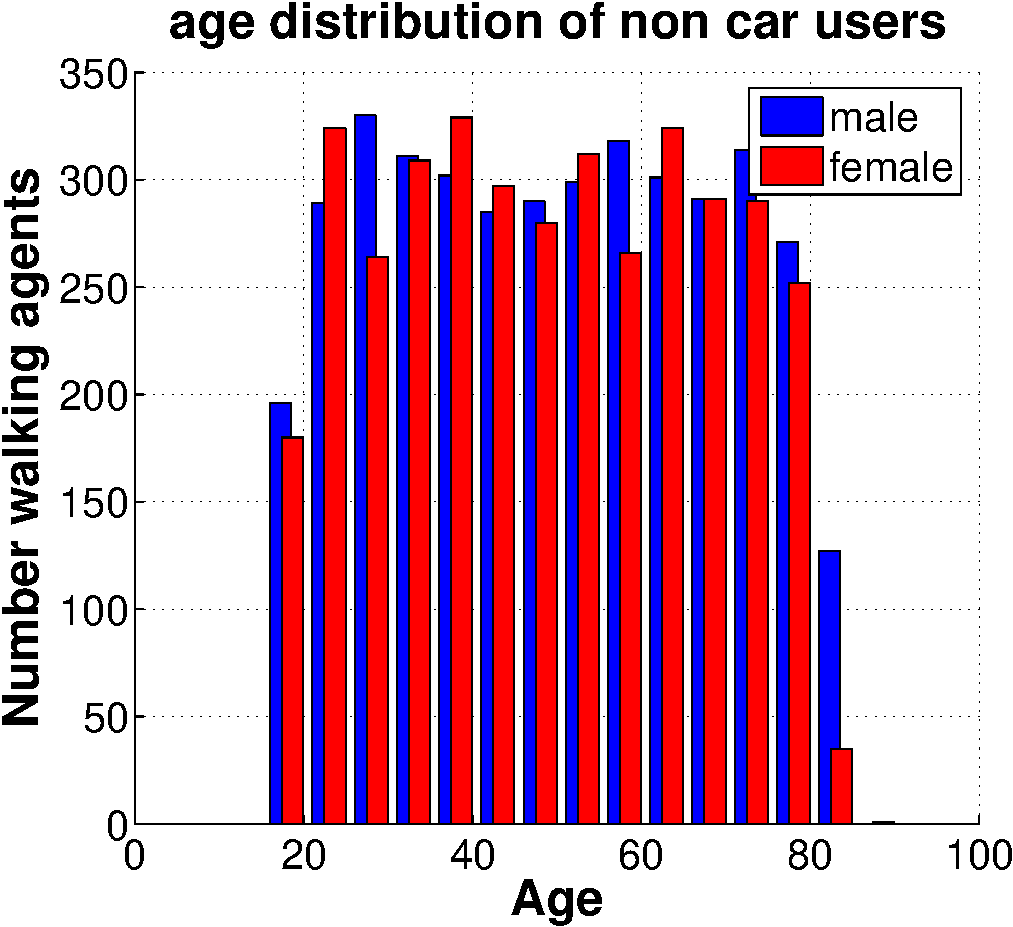
\includegraphics[width=0.47\textwidth, angle=0, trim=0mm 0mm 0mm 9mm, clip=true]{extending/figures/MultiModalSimulation/simulations/age_distribution_scatter_500}}%
  {\label{}}%
  {\hspace{3mm}}%
  \createsubfigure%
  {Capacity 1000 veh/h}%
  {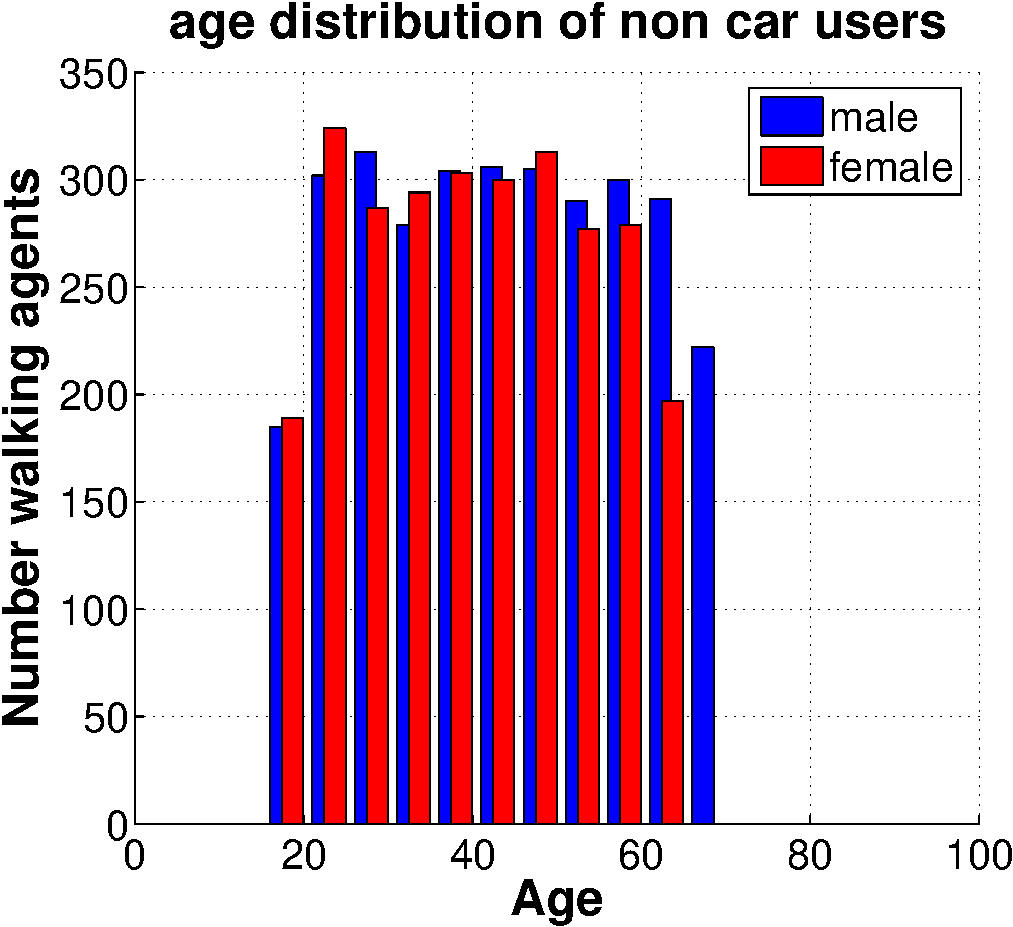
\includegraphics[width=0.47\textwidth, angle=0, trim=0mm 0mm 0mm 9mm, clip=true]{extending/figures/MultiModalSimulation/simulations/age_distribution_scatter_1000}}%
  {\label{}}%
  {\vspace{5.5mm}}%

  \createsubfigure%
  {Capacity 1500 veh/h}%
  {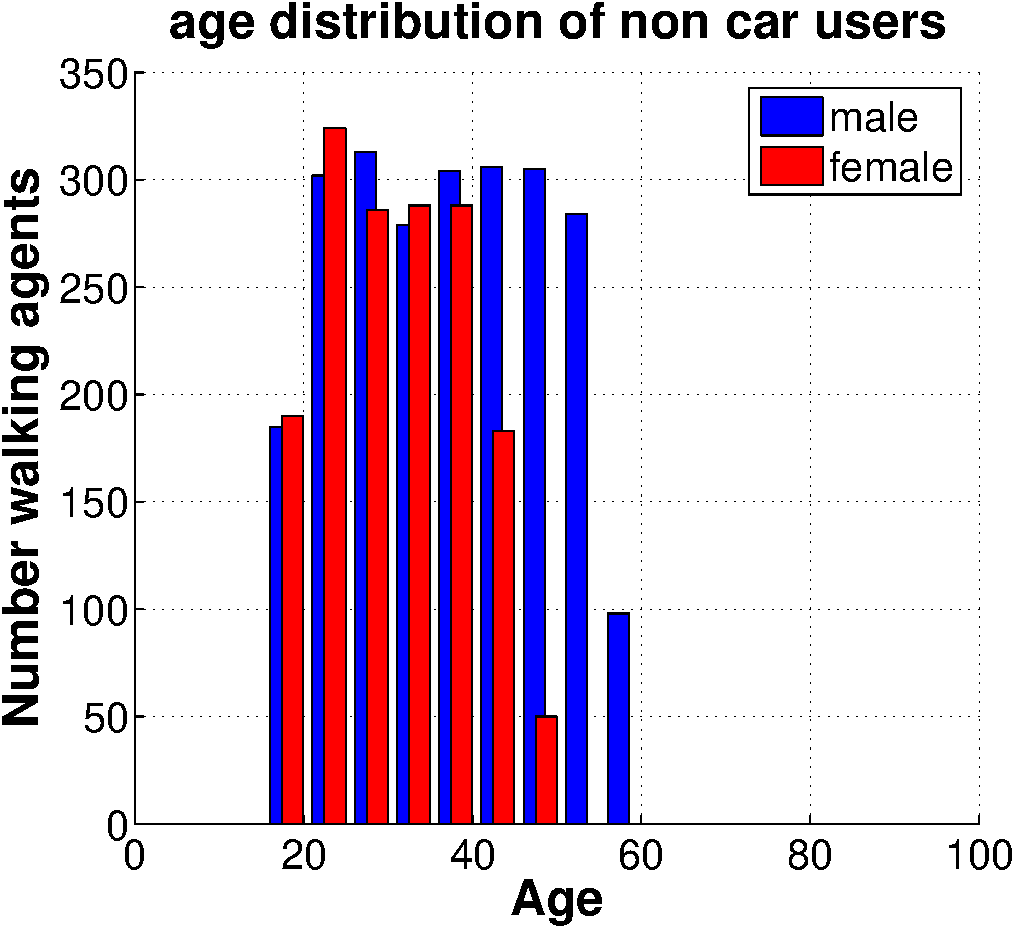
\includegraphics[width=0.47\textwidth, angle=0, trim=0mm 0mm 0mm 9mm, clip=true]{extending/figures/MultiModalSimulation/simulations/age_distribution_scatter_1500}}%
  {\label{}}%
  {\hspace{3mm}}%
  \createsubfigure%
  {Capacity 2000 veh/h}%
  {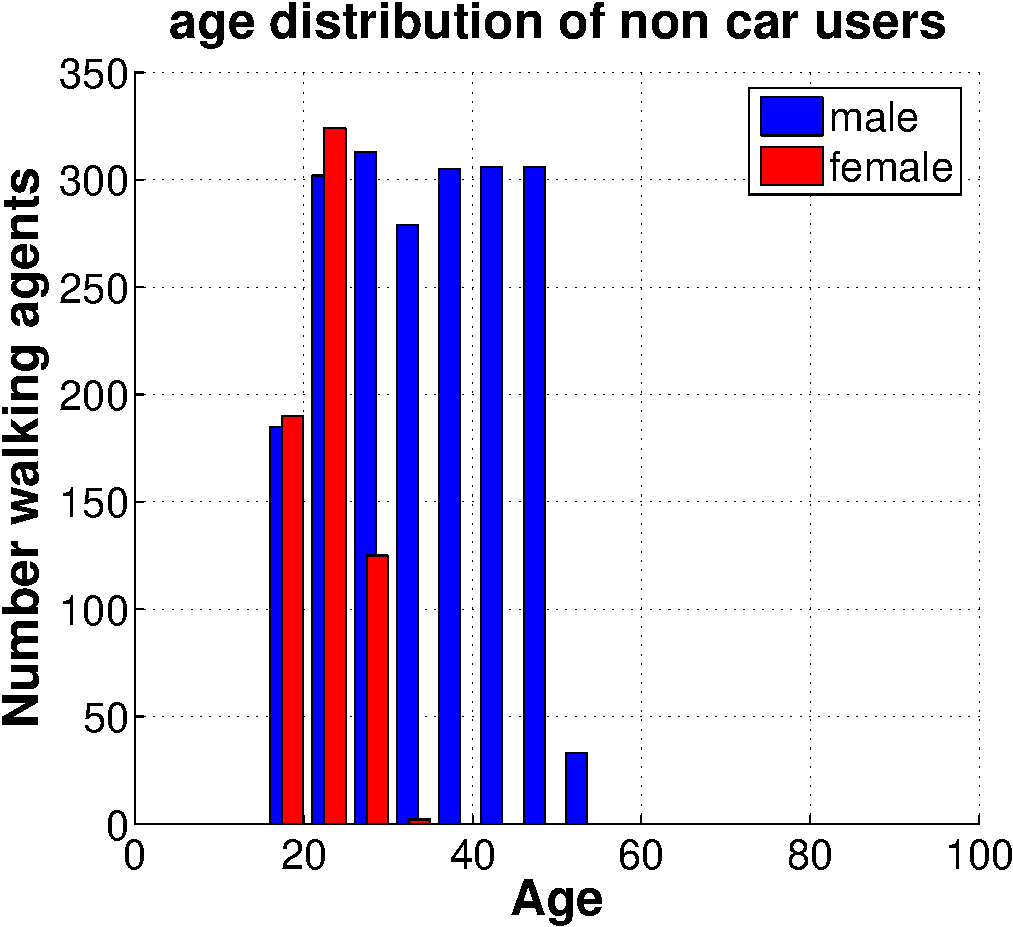
\includegraphics[width=0.47\textwidth, angle=0, trim=0mm 0mm 0mm 9mm, clip=true]{extending/figures/MultiModalSimulation/simulations/age_distribution_scatter_2000}}%
  {\label{}}%
  {\vspace{5.5mm}}%

  \createsubfigure%
  {Capacity 2500 veh/h}%
  {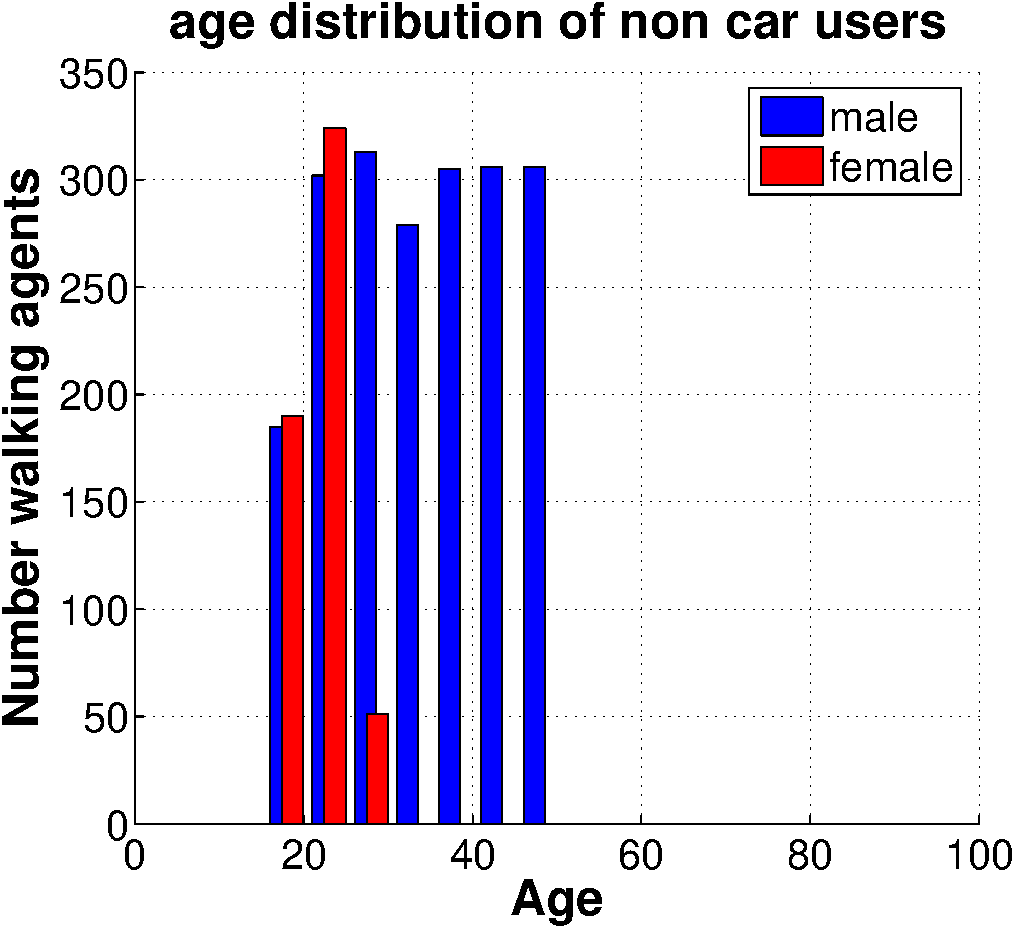
\includegraphics[width=0.47\textwidth, angle=0, trim=0mm 0mm 0mm 9mm, clip=true]{extending/figures/MultiModalSimulation/simulations/age_distribution_scatter_2500}}%
  {\label{}}%
  {\hspace{3mm}}%
  \createsubfigure%
  {Capacity unlimited}%
  {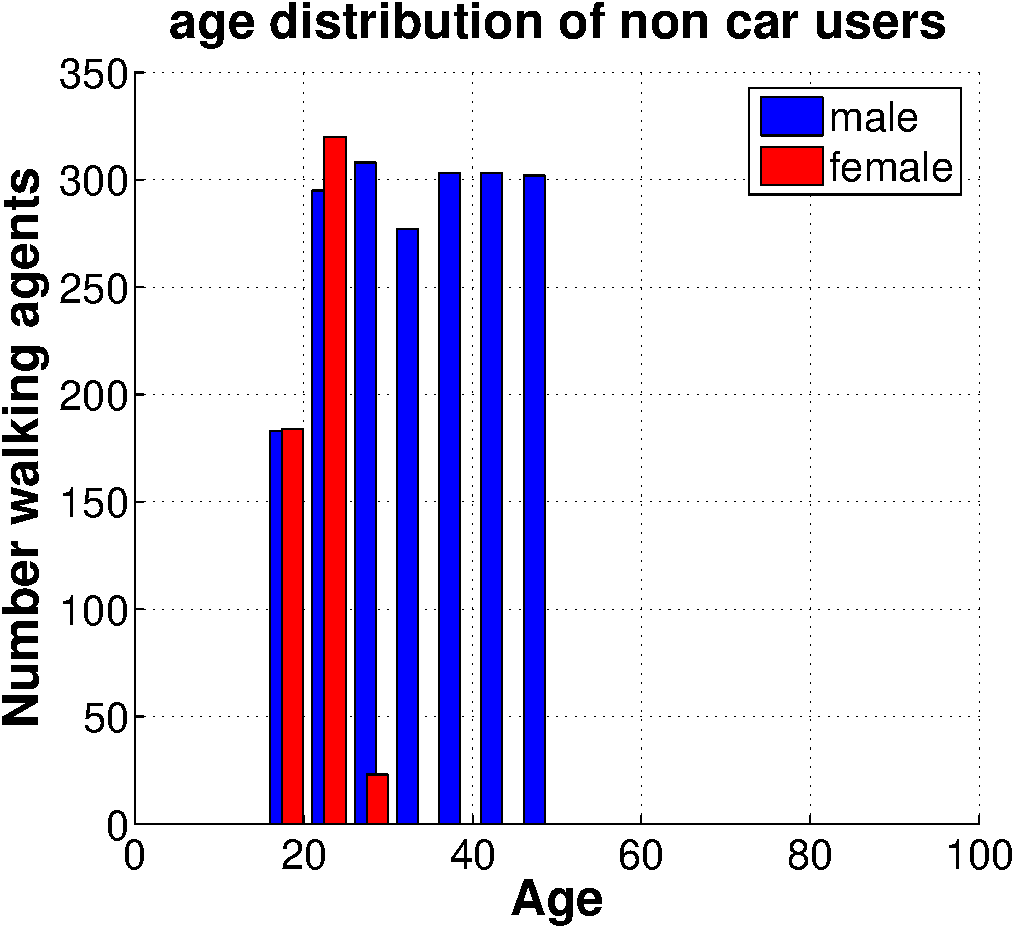
\includegraphics[width=0.47\textwidth, angle=0, trim=0mm 0mm 0mm 9mm, clip=true]{extending/figures/MultiModalSimulation/simulations/age_distribution_scatter_unlimited}}%
  {\label{}}%
  {}%
}%
{}
%---------------------------------------------------------------------

%---------------------------------------------------------------------
\createfigure%
{Influence of statistical spreading -- Age distribution with spreading}%
{Influence of statistical spreading -- Age distribution with spreading}%
{\label{fig:statisticalSpreadingAgeDistributionWithSpreading}}%
{%
  \createsubfigure%
  {Capacity 500 veh/h}%
  {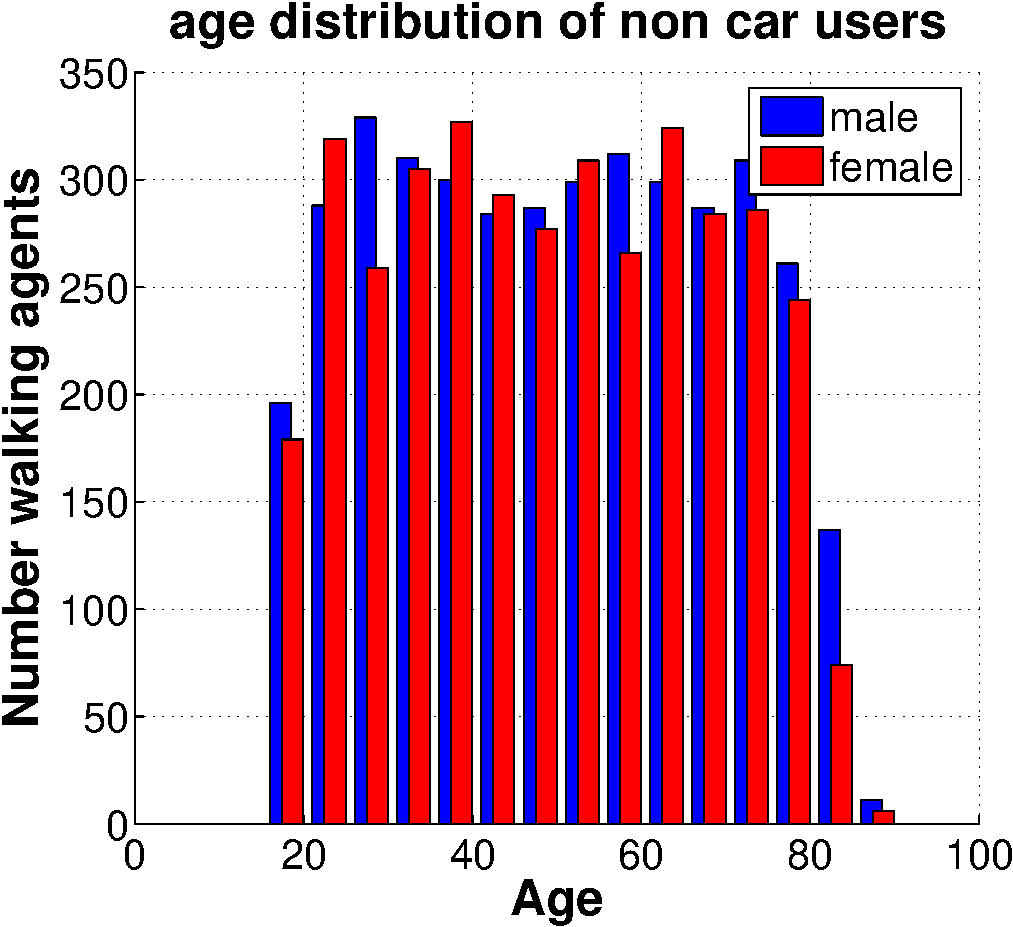
\includegraphics[width=0.47\textwidth, angle=0, trim=0mm 0mm 0mm 9mm, clip=true]{extending/figures/MultiModalSimulation/simulations/age_distribution_500}}%
  {\label{}}%
  {\hspace{3mm}}%
  \createsubfigure%
  {Capacity 1000 veh/h}%
  {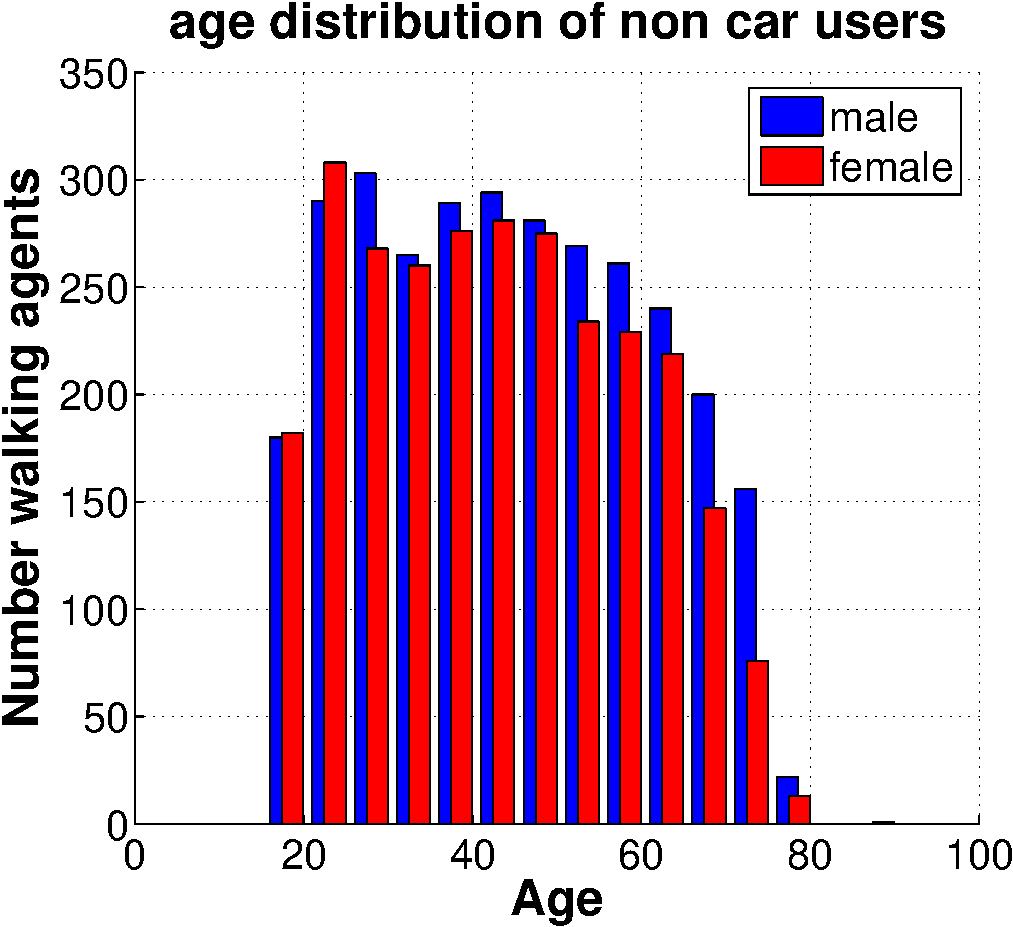
\includegraphics[width=0.47\textwidth, angle=0, trim=0mm 0mm 0mm 9mm, clip=true]{extending/figures/MultiModalSimulation/simulations/age_distribution_1000}}%
  {\label{}}%
  {\vspace{5.5mm}}%

  \createsubfigure%
  {Capacity 1500 veh/h}%
  {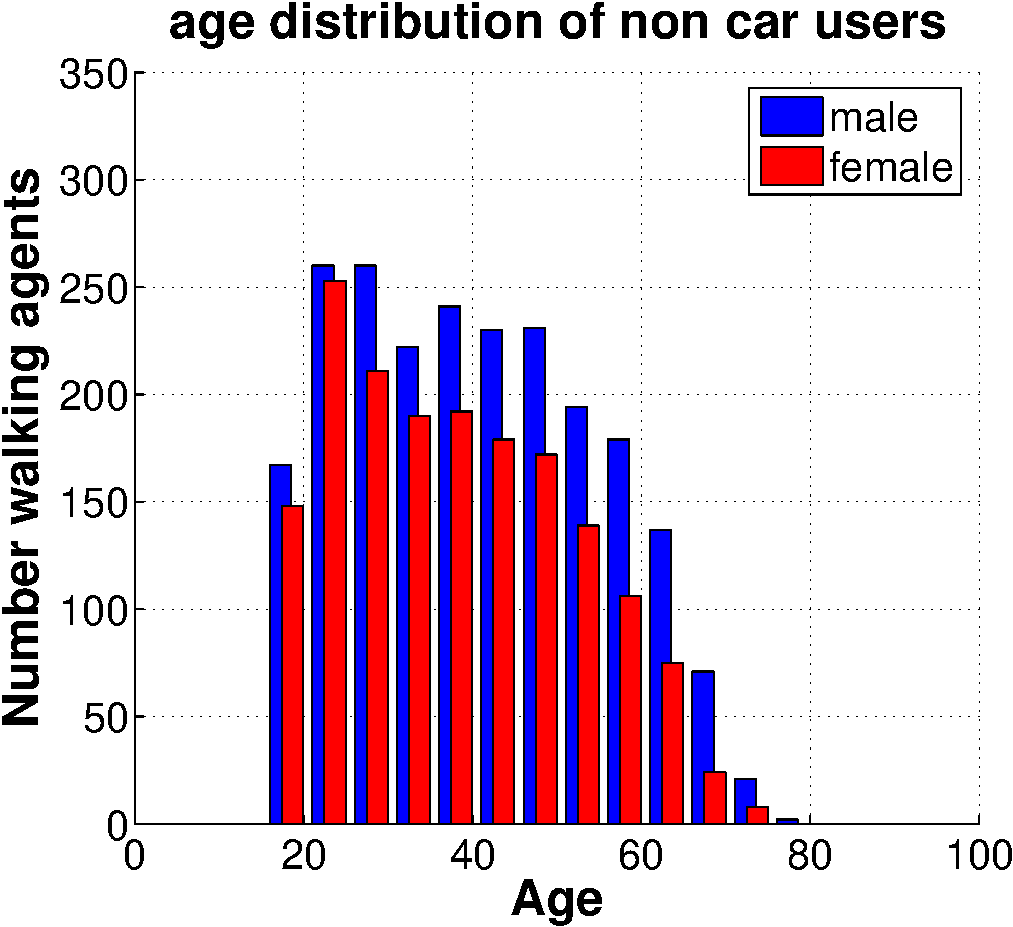
\includegraphics[width=0.47\textwidth, angle=0, trim=0mm 0mm 0mm 9mm, clip=true]{extending/figures/MultiModalSimulation/simulations/age_distribution_1500}}%
  {\label{}}%
  {\hspace{3mm}}%
  \createsubfigure%
  {Capacity 2000 veh/h}%
  {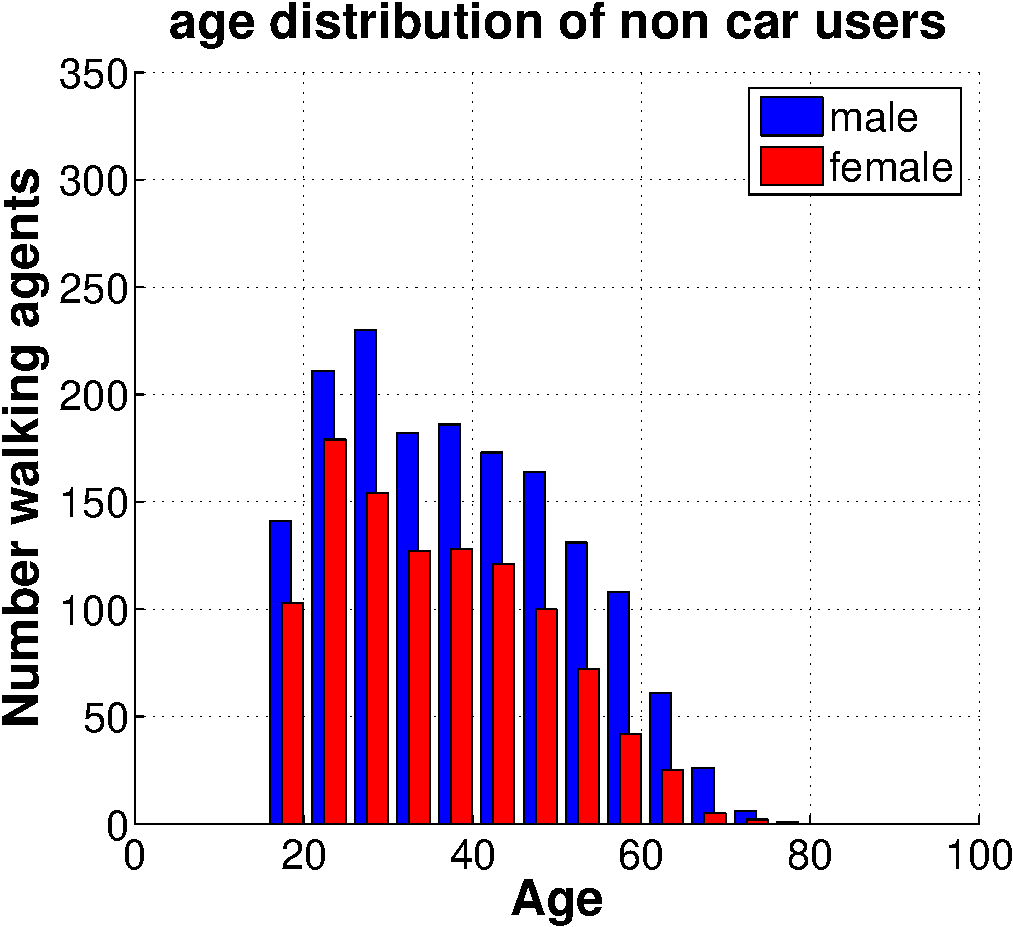
\includegraphics[width=0.47\textwidth, angle=0, trim=0mm 0mm 0mm 9mm, clip=true]{extending/figures/MultiModalSimulation/simulations/age_distribution_2000}}%
  {\label{}}%
  {\vspace{5.5mm}}%

  \createsubfigure%
  {Capacity 2500 veh/h}%
  {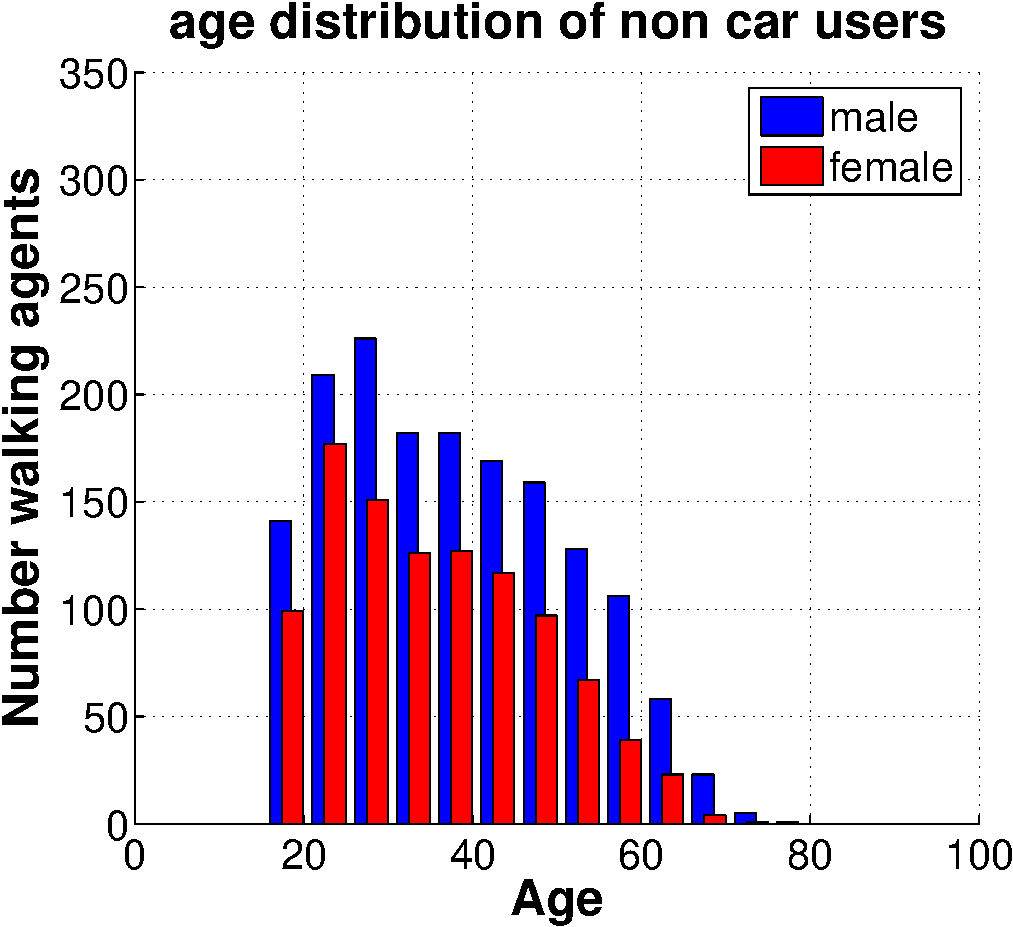
\includegraphics[width=0.47\textwidth, angle=0, trim=0mm 0mm 0mm 9mm, clip=true]{extending/figures/MultiModalSimulation/simulations/age_distribution_2500}}%
  {\label{}}%
  {\hspace{3mm}}%
  \createsubfigure%
  {Capacity unlimited}%
  {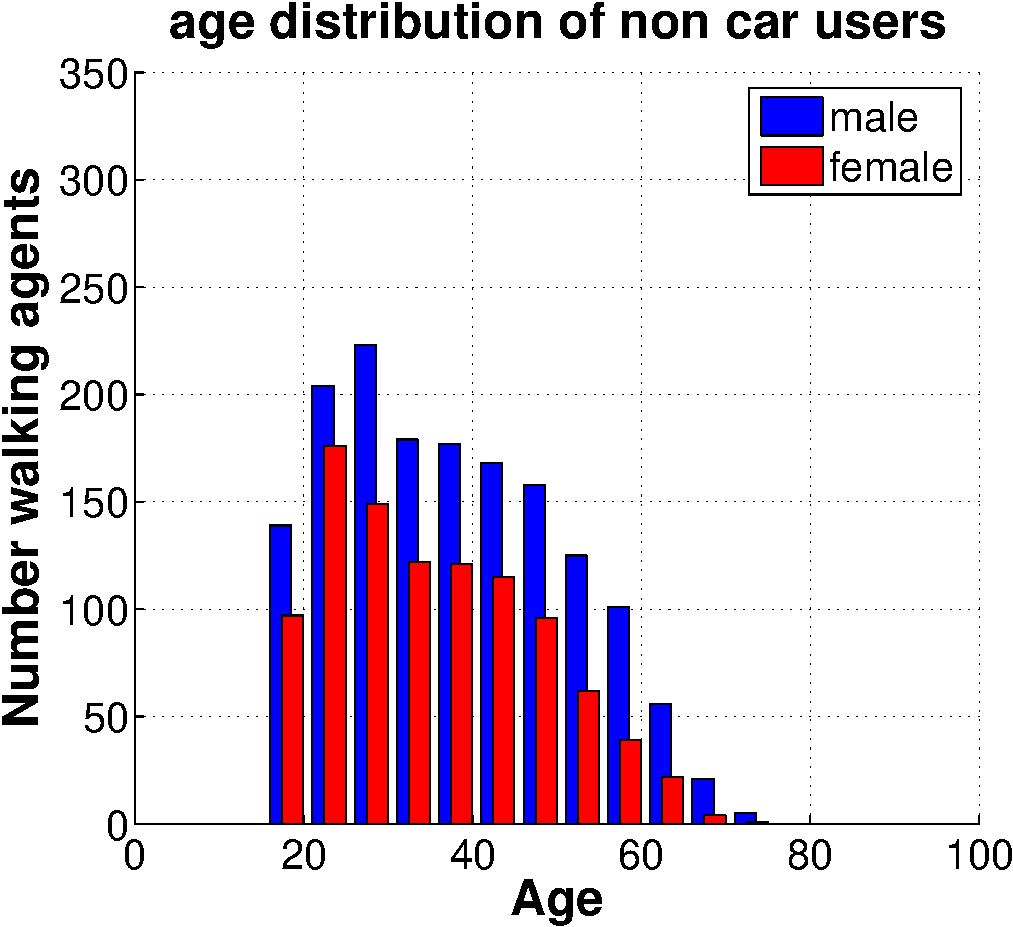
\includegraphics[width=0.45\textwidth, angle=0, trim=0mm 0mm 0mm 9mm, clip=true]{extending/figures/MultiModalSimulation/simulations/age_distribution_unlimited}}%
  {\label{}}%
  {}%
}%
{}
%---------------------------------------------------------------------

Figures \ref{fig:statisticalSpreadingAgeDistribution} and \ref{fig:statisticalSpreadingAgeDistributionWithSpreading} show the age distribution---separated into male and female---of all agents chose walking. As expected, the lower the capacity of route~1, the more agents prefer walking over going by car. The results indicate that enabling statistical spreading broadens and flattens the distribution significantly. 

The reason of this effect is depicted in Figure \ref{fig:statisticalSpreadingDistributionShape}. The figure shows how the age span which would prefer walking changes if the average walk speed is increased respectively decreased by 10\%.

%---------------------------------------------------------------------
\createfigure%
{Influence of statistical spreading -- Gender-related effects}%
{Influence of statistical spreading -- Gender-related effects}%
{\label{fig:statisticalSpreadingDistributionShape}}%
{%
  \createsubfigure%
  {Men}%
  {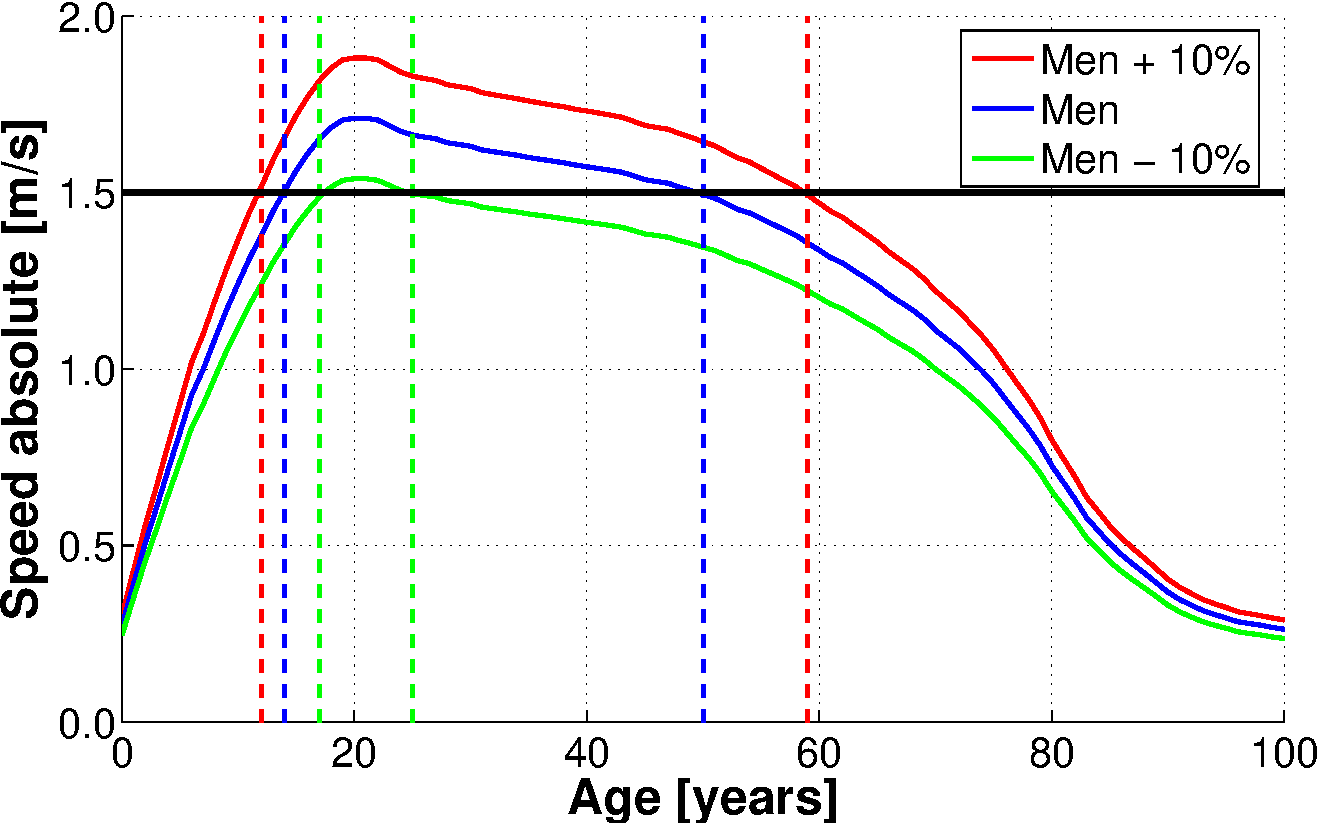
\includegraphics[width=0.80\textwidth, angle=0]{extending/figures/MultiModalSimulation/pedestrianSpeedVariationMen}}%
  {\label{fig:walkingPeople1.5}}%
  {\vspace{7.5mm}}%

  \createsubfigure%
  {Women}%
  {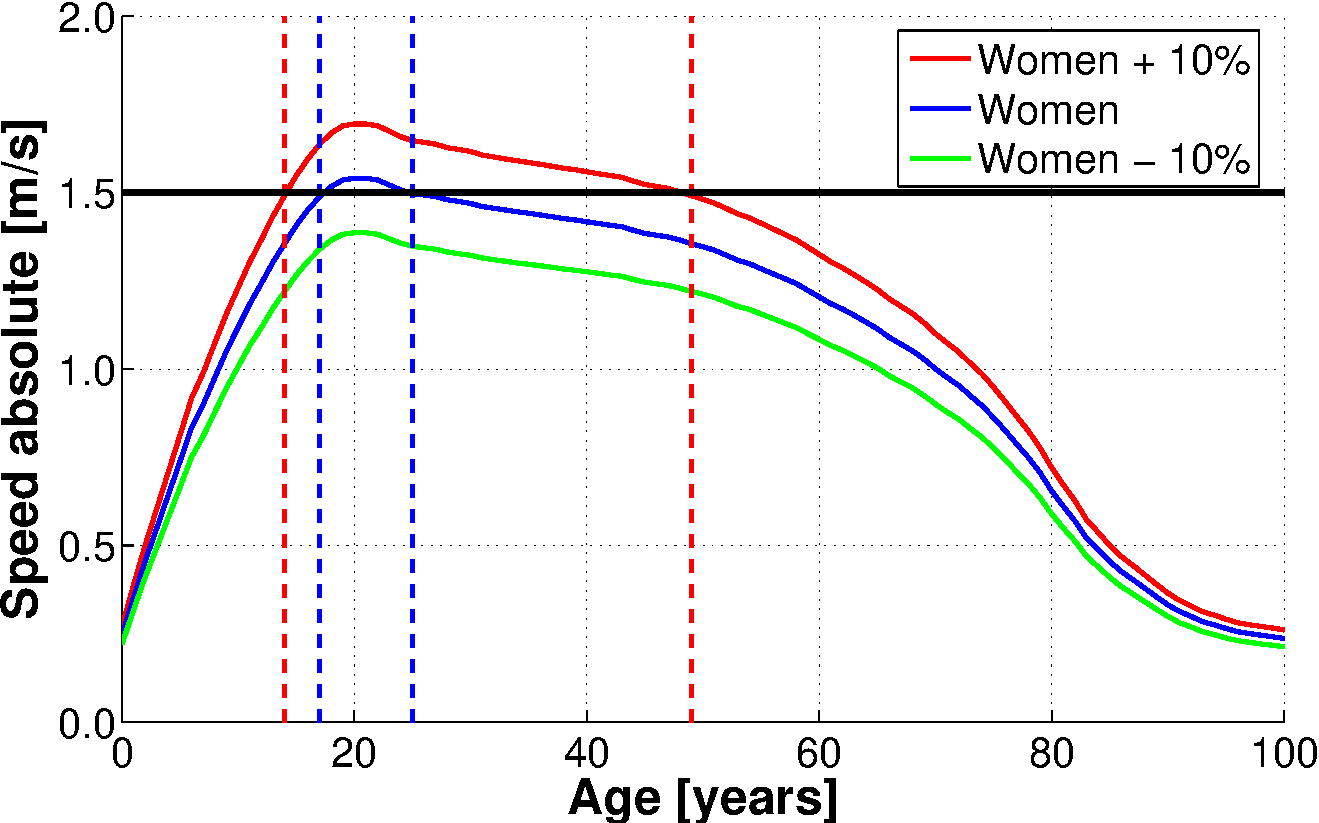
\includegraphics[width=0.80\textwidth, angle=0]{extending/figures/MultiModalSimulation/pedestrianSpeedVariationWomen}}%
  {\label{fig:walkingPeople1.0}}%
  {}%
}%
{}
%---------------------------------------------------------------------

Without statistical spreading, all people within a certain age range will prefer walking over taking the car. When people's walk speeds are scattered, some of the people within this age range will walk even faster while others will be slower than the average speed. As a result, some of those slower people might switch to using the car since that becomes the faster mode of transport for them. For people with an age that is not included in the age range which prefers walking, the effect is exactly the opposite. By default, those people prefer going by car. When a scatter factor is added to their walk speeds, some of them might switch to walking.

As shown in Figure \ref{fig:statisticalSpreadingShareWalkingAgents}, men and women are affected differently by this effect. While the share of male walking agents decreases when statistical spreading is added to the people's walk speeds, the share of female walking agents increases. Again, this finding can be explained with Figure \ref{fig:statisticalSpreadingDistributionShape}. The vertical dashed lines mark the age span of the speed profile with the same colour.  When using a reference speed of 1.5 m/s, the default age span of walking agents is 36 years (14 to 50) for men respectively 8 years (17 to 25) for women. Table \ref{tab:ageSpans} shows how the age spans changes for agents with a 10\% increased or decreased walking speed. Besides the age spans, also the absolute and relative changes are included.

%---------------------------------------------------------------------
\createtable%
{Age spans of walking agents}%
{Age spans of walking agents}%
{\label{tab:ageSpans}}%
{%
    \begin{tabular}{c|c|c|c}
       & default speed & increased by 10\% & decreased by 10\% \\
    \midrule
    \multirow{3}[0]{*}{men} & \multirow{3}[0]{*}{36 (14 - 50)} & 47 (12 - 59) & 8 (17 - 25) \\
          &       & +11   & -28 \\
          &       & +31\%  & -78\% \\
    \midrule
    \multirow{3}[0]{*}{women} & \multirow{3}[0]{*}{8 (17 - 25)} & 35 (14 - 49) & 0 (-) \\
          &       & +27   & -8 \\
          &       & +338\% & -100\% \\
    \end{tabular}%
}%
{}
%---------------------------------------------------------------------

\begin{comment}
Matlab Results:
men age 14 - 50
men plus age 12 - 59
men minus age 17 - 25
women age 17 - 25
women plus age 14 - 49
women minus age 0 - 0
\end{comment}

For male agents, the decrase (in years) is higher than the increase. In contrast, for female agents it is the other way round, which leads to the observed behaviour.

%---------------------------------------------------------------------
\createfigure%
{Influence of statistical spreading -- Share of walking agents}%
{Influence of statistical spreading -- Share of walking agents}%
{\label{fig:statisticalSpreadingShareWalkingAgents}}%
{%
  \createsubfigure%
  {Male and female - with statistical spreading}%
  {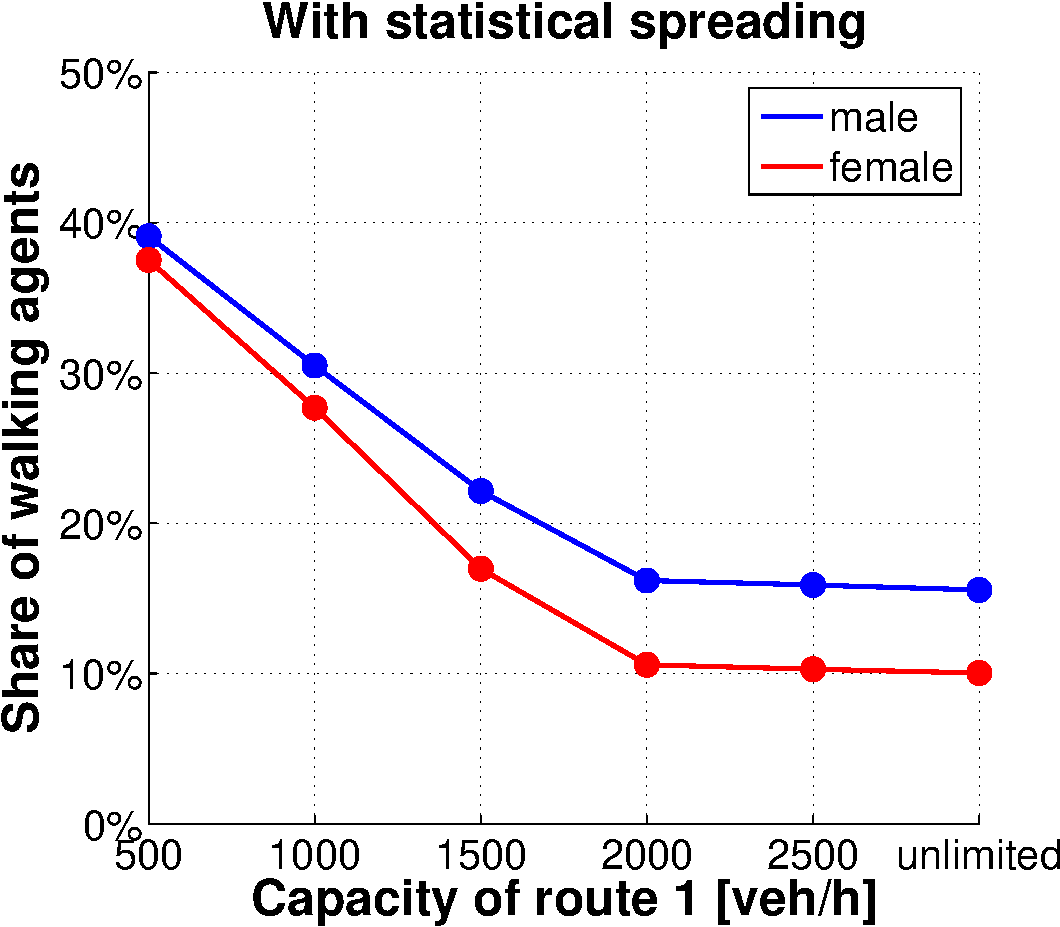
\includegraphics[width=0.48\textwidth, angle=0, trim=0mm 0mm 0mm 9mm, clip=true]{extending/figures/MultiModalSimulation/simulations/MaleAndFemaleWith}}%
  {\label{}}%
  {\hspace{3mm}}%
  \createsubfigure%
  {Male and female - without statistical spreading}%
  {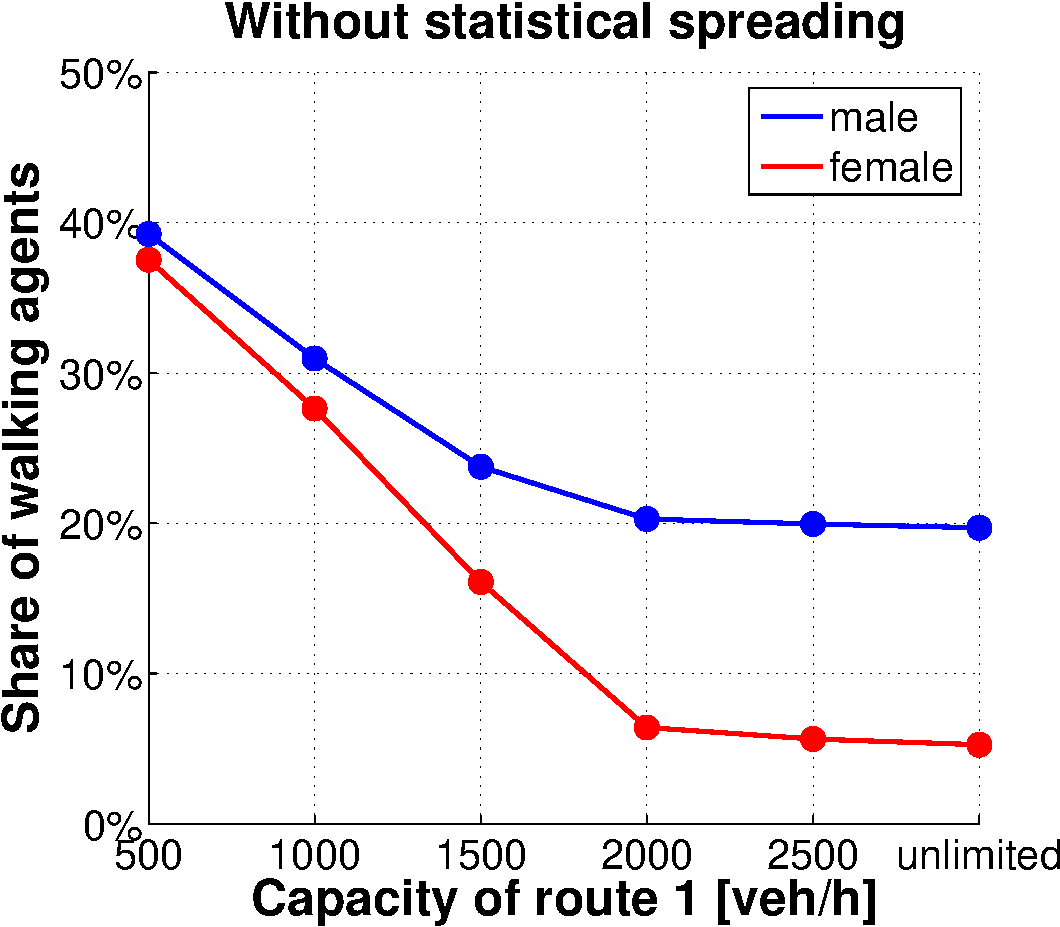
\includegraphics[width=0.48\textwidth, angle=0, trim=0mm 0mm 0mm 9mm, clip=true]{extending/figures/MultiModalSimulation/simulations/MaleAndFemaleWithout}}%
  {\label{}}%
  {\vspace{5mm}}%

  \createsubfigure%
  {With and without statistical spreading - Male}%
  {\includegraphics[width=0.48\textwidth, angle=0, trim=0mm 0mm 0mm 9mm, clip=true]{extending/figures/MultiModalSimulation/simulations/WithAndWithoutMale}}%
  {\label{}}%
  {\hspace{3mm}}%
  \createsubfigure%
  {With and without statistical spreading - Female}%
  {\includegraphics[width=0.48\textwidth, angle=0, trim=0mm 0mm 0mm 9mm, clip=true]{extending/figures/MultiModalSimulation/simulations/WithAndWithoutFemale}}%
  {\label{}}%
  {}%
}%
{}
%---------------------------------------------------------------------


%---------------------------------------------------------------------
\createfigure%
{Influence of statistical spreading -- Compare male and female results}%
{Influence of statistical spreading -- Compare male and female results}%
{\label{fig:statisticalSpreadingMaleAndFemale}}%
{%
  \createsubfigure%
  {People with walking speed $\geq$ 1.5 m/s}%
  {\includegraphics[width=0.75\textwidth, angle=0]{extending/figures/MultiModalSimulation/pedestriansAge1_5}}%
  {\label{fig:walkingPeople1.5}}%
  {\vspace{7.5mm}}%

  \createsubfigure%
  {People with walking speed $\geq$ 1.0 m/s}%
  {\includegraphics[width=0.75\textwidth, angle=0]{extending/figures/MultiModalSimulation/pedestriansAge1_0}}%
  {\label{fig:walkingPeople1.0}}%
  {\vspace{3mm}}%
}%
{}
%---------------------------------------------------------------------

Another finding from Figure \ref{fig:statisticalSpreadingShareWalkingAgents} is that the smaller the capacity of route~1, the smaller the difference between the shares of male and female agents using walk mode. This phenomena can be explained with Figure \ref{fig:statisticalSpreadingMaleAndFemale}. The two subfigures show the age groups which walk faster than 1.5 respectively 1.0~m/s. The subfigure showing people which walk faster than 1.5~m/s represents the scenario where the capacity of route~1 is not restricted. When the capacity is reduced (and as a result the car travel times increase), people with a lower walking speed (e.g.~1.0~m/s as in the second subfigure) are willing to walk. While the size of both age groups differs significantly in the first case (1.5~m/s; 8 vs.~36 years), it is comparable in the later case (1.0~m/s; 62 vs.~67 years).

%While the size of both groups is comparable in the later case (62 vs.~67 years), it differs significantly in the first case (8 vs.~36 years).


%Subfigures \ref{fig:walkingPeople1.5} and \ref{fig:walkingPeople1.0} which male and female age groups walk faster than 1.5 respectively 1.0~m/s. While the size of both groups is comparable in the later case, it differs significantly in the first case.

%- male and female interaction!\\
%- test male alone; female alone?\\


\begin{comment}
expected men share 81.818%
expected women share 18.182%
min women age 17
max women age 25
min men age 14
max men age 50
expected men share 81.818%
expected women share 18.182%
min women age 8
max women age 70
min men age 7
max men age 74
expected men share 51.938%
expected women share 48.062%
\end{comment}



%Comparing the results of runs with and without statistical spreading enabled indicates that the distribution is significantly broader.
%When adding statistical spreading is endabled, the distribution becomes wider.




%%%%%%%%%%%%%%%%%%%%%%%%%%%%%%%%%%%%%%%%%%%%%%%%%%%%%%%%%%%%%%%%%%%%%%
\subsection{Initial Transport Modes}
%%%%%%%%%%%%%%%%%%%%%%%%%%%%%%%%%%%%%%%%%%%%%%%%%%%%%%%%%%%%%%%%%%%%%%

To analyze whether the agents' initially selected transport modes influence the simulation results, a second set of experiments is conducted. The three settings used for the agent's initial transport modes are \textit{100\% car}, \textit{random selection (i.e.\ 50\% car and 50\% walk)} and \textit{100\% walk}. For each setting, six simulation runs with different capacities of route~1 are performed. Results of these runs are shown in Figures \ref{fig:InitialModeAverageCarTravelTime} to \ref{fig:InitialModeAverageNumWalkTrips}. The figures show for each simulation run the average trip travel time as well as the number of conducted trips for both transport modes.

The results demonstrate that the number of trips and the average travel times are not influenced by the agents' initially chosen transport modes. Comparing the average car and walk travel times shows that the later ones are shorter. This makes sense since agents who decide to go by foot are at least as fast agents who go by car. As a result, the average walk travel time is shorter than the average car travel time. 
%since most of the walking agents are faster than the average car travel time.

%Figure \textbf{C} depicts the mode shares ...
%As expected, the number of agent choose walking increases when the road capacity is reduced.

%Figure \textbf{D} shows the average travel time for the two modes. The average walk travel times are lower than the car travel times which is meaningful since agents decide to walk if...

\begin{comment}
- compare different start shares\\
- compare with and without scatter\\
- mode shares\\
- travel times\\
- initial mode has no influcence\\
- capacity has influence as expected\\
- histograms\\
- male vs. female share\\
\end{comment}


%---------------------------------------------------------------------
\createfigure%
{Average car travel times}%
{Average car travel times}%
{\label{fig:InitialModeAverageCarTravelTime}}%
{%
  \createsubfigure%
  {Capacity 500 veh/h}%
  {\includegraphics[width=0.47\textwidth, angle=0, trim=0mm 0mm 0mm 9mm, clip=true]{extending/figures/MultiModalSimulation/simulations/avg_car_traveltime_500}}%
  {\label{}}%
  {\hspace{3mm}}%
  \createsubfigure%
  {Capacity 1000 veh/h}%
  {\includegraphics[width=0.47\textwidth, angle=0, trim=0mm 0mm 0mm 9mm, clip=true]{extending/figures/MultiModalSimulation/simulations/avg_car_traveltime_1000}}%
  {\label{}}%
  {\vspace{7.5mm}}%

  \createsubfigure%
  {Capacity 1500 veh/h}%
  {\includegraphics[width=0.47\textwidth, angle=0, trim=0mm 0mm 0mm 9mm, clip=true]{extending/figures/MultiModalSimulation/simulations/avg_car_traveltime_1500}}%
  {\label{}}%
  {\hspace{3mm}}%
  \createsubfigure%
  {Capacity 2000 veh/h}%
  {\includegraphics[width=0.47\textwidth, angle=0, trim=0mm 0mm 0mm 9mm, clip=true]{extending/figures/MultiModalSimulation/simulations/avg_car_traveltime_2000}}%
  {\label{}}%
  {\vspace{7.5mm}}%

  \createsubfigure%
  {Capacity 2500 veh/h}%
  {\includegraphics[width=0.47\textwidth, angle=0, trim=0mm 0mm 0mm 9mm, clip=true]{extending/figures/MultiModalSimulation/simulations/avg_car_traveltime_2500}}%
  {\label{}}%
  {\hspace{3mm}}%
  \createsubfigure%
  {Capacity unlimited}%
  {\includegraphics[width=0.47\textwidth, angle=0, trim=0mm 0mm 0mm 9mm, clip=true]{extending/figures/MultiModalSimulation/simulations/avg_car_traveltime_unlimited}}%
  {\label{}}%
  {}%
}%
{}
%---------------------------------------------------------------------

%---------------------------------------------------------------------
\createfigure%
{Average walk travel times}%
{Average walk travel times}%
{\label{fig:InitialModeAverageWalkTravelTime}}%
{%
  \createsubfigure%
  {Capacity 500 veh/h}%
  {\includegraphics[width=0.47\textwidth, angle=0, trim=0mm 0mm 0mm 9mm, clip=true]{extending/figures/MultiModalSimulation/simulations/avg_walk_traveltime_500}}%
  {\label{}}%
  {\hspace{3mm}}%
  \createsubfigure%
  {Capacity 1000 veh/h}%
  {\includegraphics[width=0.47\textwidth, angle=0, trim=0mm 0mm 0mm 9mm, clip=true]{extending/figures/MultiModalSimulation/simulations/avg_walk_traveltime_1000}}%
  {\label{}}%
  {\vspace{7.5mm}}%

  \createsubfigure%
  {Capacity 1500 veh/h}%
  {\includegraphics[width=0.47\textwidth, angle=0, trim=0mm 0mm 0mm 9mm, clip=true]{extending/figures/MultiModalSimulation/simulations/avg_walk_traveltime_1500}}%
  {\label{}}%
  {\hspace{3mm}}%
  \createsubfigure%
  {Capacity 2000 veh/h}%
  {\includegraphics[width=0.47\textwidth, angle=0, trim=0mm 0mm 0mm 9mm, clip=true]{extending/figures/MultiModalSimulation/simulations/avg_walk_traveltime_2000}}%
  {\label{}}%
  {\vspace{7.5mm}}%

  \createsubfigure%
  {Capacity 2500 veh/h}%
  {\includegraphics[width=0.47\textwidth, angle=0, trim=0mm 0mm 0mm 9mm, clip=true]{extending/figures/MultiModalSimulation/simulations/avg_walk_traveltime_2500}}%
  {\label{}}%
  {\hspace{3mm}}%
  \createsubfigure%
  {Capacity unlimited}%
  {\includegraphics[width=0.47\textwidth, angle=0, trim=0mm 0mm 0mm 9mm, clip=true]{extending/figures/MultiModalSimulation/simulations/avg_walk_traveltime_unlimited}}%
  {\label{}}%
  {}%
}%
{}
%---------------------------------------------------------------------

%---------------------------------------------------------------------
\createfigure%
{Number of car trips}%
{Number of car trips}%
{\label{fig:InitialModeAverageNumCarTrips}}%
{%
  \createsubfigure%
  {Capacity 500 veh/h}%
  {\includegraphics[width=0.47\textwidth, angle=0, trim=0mm 0mm 0mm 9mm, clip=true]{extending/figures/MultiModalSimulation/simulations/num_car_trips_500}}%
  {\label{}}%
  {\hspace{3mm}}%
  \createsubfigure%
  {Capacity 1000 veh/h}%
  {\includegraphics[width=0.47\textwidth, angle=0, trim=0mm 0mm 0mm 9mm, clip=true]{extending/figures/MultiModalSimulation/simulations/num_car_trips_1000}}%
  {\label{}}%
  {\vspace{7.5mm}}%

  \createsubfigure%
  {Capacity 1500 veh/h}%
  {\includegraphics[width=0.47\textwidth, angle=0, trim=0mm 0mm 0mm 9mm, clip=true]{extending/figures/MultiModalSimulation/simulations/num_car_trips_1500}}%
  {\label{}}%
  {\hspace{3mm}}%
  \createsubfigure%
  {Capacity 2000 veh/h}%
  {\includegraphics[width=0.47\textwidth, angle=0, trim=0mm 0mm 0mm 9mm, clip=true]{extending/figures/MultiModalSimulation/simulations/num_car_trips_2000}}%
  {\label{}}%
  {\vspace{7.5mm}}%

  \createsubfigure%
  {Capacity 2500 veh/h}%
  {\includegraphics[width=0.47\textwidth, angle=0, trim=0mm 0mm 0mm 9mm, clip=true]{extending/figures/MultiModalSimulation/simulations/num_car_trips_2500}}%
  {\label{}}%
  {\hspace{3mm}}%
  \createsubfigure%
  {Capacity unlimited}%
  {\includegraphics[width=0.47\textwidth, angle=0, trim=0mm 0mm 0mm 9mm, clip=true]{extending/figures/MultiModalSimulation/simulations/num_car_trips_unlimited}}%
  {\label{}}%
  {}%
}%
{}
%---------------------------------------------------------------------

%---------------------------------------------------------------------
\createfigure%
{Number of walk trips}%
{Number of walk trips}%
{\label{fig:InitialModeAverageNumWalkTrips}}%
{%
  \createsubfigure%
  {Capacity 500 veh/h}%
  {\includegraphics[width=0.47\textwidth, angle=0, trim=0mm 0mm 0mm 9mm, clip=true]{extending/figures/MultiModalSimulation/simulations/num_walk_trips_500}}%
  {\label{}}%
  {\hspace{3mm}}%
  \createsubfigure%
  {Capacity 1000 veh/h}%
  {\includegraphics[width=0.47\textwidth, angle=0, trim=0mm 0mm 0mm 9mm, clip=true]{extending/figures/MultiModalSimulation/simulations/num_walk_trips_1000}}%
  {\label{}}%
  {\vspace{7.5mm}}%

  \createsubfigure%
  {Capacity 1500 veh/h}%
  {\includegraphics[width=0.47\textwidth, angle=0, trim=0mm 0mm 0mm 9mm, clip=true]{extending/figures/MultiModalSimulation/simulations/num_walk_trips_1500}}%
  {\label{}}%
  {\hspace{3mm}}%
  \createsubfigure%
  {Capacity 2000 veh/h}%
  {\includegraphics[width=0.47\textwidth, angle=0, trim=0mm 0mm 0mm 9mm, clip=true]{extending/figures/MultiModalSimulation/simulations/num_walk_trips_2000}}%
  {\label{}}%
  {\vspace{7.5mm}}%

  \createsubfigure%
  {Capacity 2500 veh/h}%
  {\includegraphics[width=0.47\textwidth, angle=0, trim=0mm 0mm 0mm 9mm, clip=true]{extending/figures/MultiModalSimulation/simulations/num_walk_trips_2500}}%
  {\label{}}%
  {\hspace{3mm}}%
  \createsubfigure%
  {Capacity unlimited}%
  {\includegraphics[width=0.47\textwidth, angle=0, trim=0mm 0mm 0mm 9mm, clip=true]{extending/figures/MultiModalSimulation/simulations/num_walk_trips_unlimited}}%
  {\label{}}%
  {}%
}%
{}
%---------------------------------------------------------------------

% ##################################################################################################################
\section{Conclusions}
This chapter introduced an extension of MATSim's transport micro-simulation which adds support non-motorized trips to the framework. it allow tracking an agent's movement in detail, which is one essential requirement for studies related to topics like evacuations, e-bikes, car sharing or public transport.

A first implementation of a pedestrian simulation module for MATSim which also supports agent-agent interactions has been presented by \citet{LaemmelPlaue_PED_2012}. Due to the high computational effort of the underlying physical model, the scenario size is limited to a few thousand agents. An experimental combination of their implementation and the module for non-vehicular traffic is described by \citet{DoblerLaemmel_PED_2012}. This combined implementation allows to simluate regions of a scenario with many pedestrians with a high resolution model while other regions are simulated with the faster but less detailed approach.

% ##################################################################################################################